%==============================================================================
% tento soubor pouzijte jako zaklad
% this file should be used as a base for the thesis
% Autoři / Authors: 2008 Michal Bidlo, 2019 Jaroslav Dytrych
% Kontakt pro dotazy a připomínky: sablona@fit.vutbr.cz
% Contact for questions and comments: sablona@fit.vutbr.cz
%==============================================================================
% kodovani: UTF-8 (zmena prikazem iconv, recode nebo cstocs)
% encoding: UTF-8 (you can change it by command iconv, recode or cstocs)
%------------------------------------------------------------------------------
% zpracování / processing: make, make pdf, make clean
%==============================================================================
% Soubory, které je nutné upravit nebo smazat: / Files which have to be edited or deleted:
%   xhrusk25-slack-api-headless-cms-20-literatura-bibliography.bib - literatura / bibliography
%   xhrusk25-slack-api-headless-cms-01-kapitoly-chapters.tex - obsah práce / the thesis content
%   xhrusk25-slack-api-headless-cms-01-kapitoly-chapters-en.tex - obsah práce v angličtině / the thesis content in English
%   xhrusk25-slack-api-headless-cms-30-prilohy-appendices.tex - přílohy / appendices
%   xhrusk25-slack-api-headless-cms-30-prilohy-appendices-en.tex - přílohy v angličtině / appendices in English
%==============================================================================
\documentclass[slovak, zadani]{fitthesis} % bez zadání - pro začátek práce, aby nebyl problém s překladem
%\documentclass[english]{fitthesis} % without assignment - for the work start to avoid compilation problem
%\documentclass[zadani]{fitthesis} % odevzdani do wisu a/nebo tisk s barevnými odkazy - odkazy jsou barevné
%\documentclass[english,zadani]{fitthesis} % for submission to the IS FIT and/or print with color links - links are color
%\documentclass[zadani,print]{fitthesis} % pro černobílý tisk - odkazy jsou černé
%\documentclass[english,zadani,print]{fitthesis} % for the black and white print - links are black
%\documentclass[zadani,cprint]{fitthesis} % pro barevný tisk - odkazy jsou černé, znak VUT barevný
%\documentclass[english,zadani,cprint]{fitthesis} % for the print - links are black, logo is color
% * Je-li práce psaná v anglickém jazyce, je zapotřebí u třídy použít 
%   parametr english následovně:
%   If thesis is written in English, it is necessary to use 
%   parameter english as follows:
%      \documentclass[english]{fitthesis}
% * Je-li práce psaná ve slovenském jazyce, je zapotřebí u třídy použít 
%   parametr slovak následovně:
%   If the work is written in the Slovak language, it is necessary 
%   to use parameter slovak as follows:
%      \documentclass[slovak]{fitthesis}
% * Je-li práce psaná v anglickém jazyce se slovenským abstraktem apod., 
%   je zapotřebí u třídy použít parametry english a enslovak následovně:
%   If the work is written in English with the Slovak abstract, etc., 
%   it is necessary to use parameters english and enslovak as follows:
%      \documentclass[english,enslovak]{fitthesis}

% Základní balíčky jsou dole v souboru šablony fitthesis.cls
% Basic packages are at the bottom of template file fitthesis.cls
% zde můžeme vložit vlastní balíčky / you can place own packages here

% Kompilace po částech (rychlejší, ale v náhledu nemusí být vše aktuální)
% Compilation piecewise (faster, but not all parts in preview will be up-to-date)
% \usepackage{subfiles}

% Nastavení cesty k obrázkům
% Setting of a path to the pictures
%\graphicspath{{obrazky-figures/}{./obrazky-figures/}}
%\graphicspath{{obrazky-figures/}{../obrazky-figures/}}

%---rm---------------
\renewcommand{\rmdefault}{lmr}%zavede Latin Modern Roman jako rm / set Latin Modern Roman as rm
%---sf---------------
\renewcommand{\sfdefault}{qhv}%zavede TeX Gyre Heros jako sf
%---tt------------
\renewcommand{\ttdefault}{lmtt}% zavede Latin Modern tt jako tt

% vypne funkci šablony, která automaticky nahrazuje uvozovky,
% aby nebyly prováděny nevhodné náhrady v popisech API apod.
% disables function of the template which replaces quotation marks
% to avoid unnecessary replacements in the API descriptions etc.
\csdoublequotesoff

% Doplňujúce balíky
%---------------------------------------------------------------------------
\usepackage{url}
\usepackage[threshold=0]{csquotes}
\usepackage{listings}

% Farby
%---------------------------------------------------------------------------
\definecolor{codegreen}{rgb}{0.29, 0.77, 0.38}
\definecolor{codeblack}{rgb}{0, 0, 0}
\definecolor{codepurple}{rgb}{0.58, 0, 0.82}
\definecolor{backcolour}{rgb}{0.95, 0.95, 0.95}

% Štýly pre lstlisting (code)
%---------------------------------------------------------------------------
\lstdefinelanguage{TypeScript}{
  morekeywords=[1]{break, continue, delete, else, for, function, if, in, new, return, this, typeof, var, void, while, with, await, async, case, catch, class, const, default, do, enum, export, extends, finally, from, implements, import, instanceof, let, static, super, switch, throw, try, type},
  morekeywords=[2]{false, null, true, boolean, number, undefined, Array, Boolean, Date, Math, Number, string, String, Object},
  morekeywords=[3]{eval, fetch, parseInt, parseFloat, STRINGIFY},
  sensitive,
  morecomment=[s]{/*}{*/},
  morecomment=[l]//,
  morecomment=[s]{/**}{*/},
  morestring=[b]',
  morestring=[b]",
  morestring=[b]`
}[keywords, comments, strings]

\lstdefinelanguage{GraphQL}{
  morekeywords=[1]{input, type},
  morekeywords=[2]{Boolean, ID, Int, String},
  sensitive,
  morecomment=[l]\#,
  morestring=[b]"
}[keywords, comments, strings]

\lstdefinestyle{CommonCodeStyle}{
    backgroundcolor=\color{backcolour},   
    commentstyle=\color{codegreen},
    keywordstyle=\color{magenta},
    numberstyle=\tiny\color{codeblack},
    stringstyle=\color{codepurple},
    basicstyle=\ttfamily\footnotesize,
    breakatwhitespace=false,         
    breaklines=true,                 
    captionpos=b,                    
    keepspaces=true,                 
    numbers=left,                    
    numbersep=5pt,                  
    showspaces=false,                
    showstringspaces=false,
    showtabs=false,                  
    tabsize=2
}

\lstdefinestyle{TypeScript}{
  language=TypeScript,
  style=CommonCodeStyle
}

\lstdefinestyle{GraphQL}{
  language=GraphQL,
  style=CommonCodeStyle
}

\lstset{style=CommonCodeStyle, language=TypeScript}

% Delenie slov
%---------------------------------------------------------------------------
\hyphenation{PostgreSQL}
\hyphenation{JavaScript}
\hyphenation{TypeScript}

% =======================================================================
% balíček "hyperref" vytváří klikací odkazy v pdf, pokud tedy použijeme pdflatex
% problém je, že balíček hyperref musí být uveden jako poslední, takže nemůže
% být v šabloně
% "hyperref" package create clickable links in pdf if you are using pdflatex.
% Problem is that this package have to be introduced as the last one so it 
% can not be placed in the template file.
\ifWis
\ifx\pdfoutput\undefined % nejedeme pod pdflatexem / we are not using pdflatex
\else
  \usepackage{color}
  \usepackage[unicode,colorlinks,hyperindex,plainpages=false,pdftex]{hyperref}
  \definecolor{hrcolor-ref}{RGB}{223,52,30}
  \definecolor{hrcolor-cite}{HTML}{2F8F00}
  \definecolor{hrcolor-urls}{HTML}{092EAB}
  \hypersetup{
	linkcolor=hrcolor-ref,
	citecolor=hrcolor-cite,
	filecolor=magenta,
	urlcolor=hrcolor-urls
  }
  \def\pdfBorderAttrs{/Border [0 0 0] }  % bez okrajů kolem odkazů / without margins around links
  \pdfcompresslevel=9
\fi
\else % pro tisk budou odkazy, na které se dá klikat, černé / for the print clickable links will be black
\ifx\pdfoutput\undefined % nejedeme pod pdflatexem / we are not using pdflatex
\else
  \usepackage{color}
  \usepackage[unicode,colorlinks,hyperindex,plainpages=false,pdftex,urlcolor=black,linkcolor=black,citecolor=black]{hyperref}
  \definecolor{links}{rgb}{0,0,0}
  \definecolor{anchors}{rgb}{0,0,0}
  \def\AnchorColor{anchors}
  \def\LinkColor{links}
  \def\pdfBorderAttrs{/Border [0 0 0] } % bez okrajů kolem odkazů / without margins around links
  \pdfcompresslevel=9
\fi
\fi
% Řešení problému, kdy klikací odkazy na obrázky vedou za obrázek
% This solves the problems with links which leads after the picture
\usepackage[all]{hypcap}

% Informace o práci/projektu / Information about the thesis
%---------------------------------------------------------------------------
\projectinfo{
  %Prace / Thesis
  project={BP},            %typ práce BP/SP/DP/DR  / thesis type (SP = term project)
  year={2020},             % rok odevzdání / year of submission
  date=\today,             % datum odevzdání / submission date
  %Nazev prace / thesis title
  title.cs={Využití Slack API pro HeadlessCMS},  % název práce v češtině či slovenštině (dle zadání) / thesis title in czech language (according to assignment)
  title.en={Use of Slack API for HeadlessCMS}, % název práce v angličtině / thesis title in english
  %title.length={14.5cm}, % nastavení délky bloku s titulkem pro úpravu zalomení řádku (lze definovat zde nebo níže) / setting the length of a block with a thesis title for adjusting a line break (can be defined here or below)
  %sectitle.length={14.5cm}, % nastavení délky bloku s druhým titulkem pro úpravu zalomení řádku (lze definovat zde nebo níže) / setting the length of a block with a second thesis title for adjusting a line break (can be defined here or below)
  %Autor / Author
  author.name={Jozef},   % jméno autora / author name
  author.surname={Hruška},   % příjmení autora / author surname 
  %author.title.p={Bc.}, % titul před jménem (nepovinné) / title before the name (optional)
  %author.title.a={Ph.D.}, % titul za jménem (nepovinné) / title after the name (optional)
  %Ustav / Department
  department={UIFS}, % doplňte příslušnou zkratku dle ústavu na zadání: UPSY/UIFS/UITS/UPGM / fill in appropriate abbreviation of the department according to assignment: UPSY/UIFS/UITS/UPGM
  % Školitel / supervisor
  supervisor.name={Vladimír},   % jméno školitele / supervisor name 
  supervisor.surname={Bartík},   % příjmení školitele / supervisor surname
  supervisor.title.p={Ing.},   %titul před jménem (nepovinné) / title before the name (optional)
  supervisor.title.a={Ph.D.},    %titul za jménem (nepovinné) / title after the name (optional)
  % Klíčová slova / keywords
  keywords.cs={RS, Slack, React, Prisma, Apollo, Node.js, Next.js, Redux, Bolt, GraphQL, TypeScript, PostgreSQL}, % klíčová slova v českém či slovenském jazyce / keywords in czech or slovak language
  keywords.en={CMS, Slack, React, Prisma, Apollo, Node.js, Next.js, Redux, Bolt, GraphQL, TypeScript, PostgreSQL}, % klíčová slova v anglickém jazyce / keywords in english
  %keywords.en={Here, individual keywords separated by commas will be written in English.},
  % Abstrakt / Abstract
  abstract.cs={Práca si dáva za~cieľ vytvoriť redakčný systém s~otvoreným aplikačným rozhraním (Headless CMS) a~možnosťou správy obsahu v~prostredí aplikácie Slack. Inštalácia a~následné používanie systému nevyžaduje žiadnu konfiguráciu zo~strany uživateľa. Otvorené (verejné) ako aj uzatvorené (skryté) aplikačné rozhranie je vybudované podľa špecifikácie GraphQL. Otvorené rozhranie slúži výhradne k čítaniu dát, tzn. že nie je možné dáta akokoľvek vkladať či modifikovať použitím tohto rozhrania. Výstupom práce je plne funkčný prototyp systému, ktorého súčasti boli implementované pomocou nástrojov React a Node.js s dôrazom na prívetivosť uživateľského rozhrania.}, % abstrakt v českém či slovenském jazyce / abstract in czech or slovak language
  abstract.en={The aim of this thesis is~to~create a~content management system with~open application interface (Headless CMS) and~capability of~content management inside Slack application. Installation and~use of~system does not require any configuration by~user. Open (public) and~closed (hidden) application interface is~built following GraphQL specification. The opne interface is~read-only which means it~is~not possible to insert or~modify data through this interface. The output of~this work is~a~fully functional prototype implemented with tools as~React and~Node.js with focus on~user-friendly interface.}, % abstrakt v anglickém jazyce / abstract in english
  %abstract.en={An abstract of the work in English will be written in this paragraph.},
  % Prohlášení (u anglicky psané práce anglicky, u slovensky psané práce slovensky) / Declaration (for thesis in english should be in english)
  declaration={Prehlasujem, že som túto bakalársku prácu vypracoval samostatne pod vedením Ing. Vladimíra Bartíka, Ph.D.
Uviedol som všetky literárne pramene, publikácie a~ďaľšie zdroje, z~ktorých som čerpal.},
  %declaration={I hereby declare that this Bachelor's thesis was prepared as an original work by the author under the supervision of Mr. X
% The supplementary information was provided by Mr. Y
% I have listed all the literary sources, publications and other sources, which were used during the preparation of this thesis.},
  % Poděkování (nepovinné, nejlépe v jazyce práce) / Acknowledgement (optional, ideally in the language of the thesis)
  acknowledgment={Rád by som poďakoval Ing. Vladimírovi Bartíkovi, Ph.D. za odborné vedenia a~čas venovaný mojej bakalárskej práci. Ďaľej by som rád poďakoval Jánovi Vorčákovi, M.Sc., za inšpiráciu vedúcu k~téme tejto práce, za jeho cenné rady a~konzultácie.},
  %acknowledgment={Here it is possible to express thanks to the supervisor and to the people which provided professional help
%(external submitter, consultant, etc.).},
  % Rozšířený abstrakt (cca 3 normostrany) - lze definovat zde nebo níže / Extended abstract (approximately 3 standard pages) - can be defined here or below
  %extendedabstract={Do tohoto odstavce bude zapsán rozšířený výtah (abstrakt) práce v českém (slovenském) jazyce.},
  %faculty={FIT}, % FIT/FEKT/FSI/FA/FCH/FP/FAST/FAVU/USI/DEF
  faculty.cs={Fakulta informačních technologií}, % Fakulta v češtině - pro využití této položky výše zvolte fakultu DEF / Faculty in Czech - for use of this entry select DEF above
  faculty.en={Faculty of Information Technology}, % Fakulta v angličtině - pro využití této položky výše zvolte fakultu DEF / Faculty in English - for use of this entry select DEF above
  department.cs={Ústav matematiky}, % Ústav v češtině - pro využití této položky výše zvolte ústav DEF nebo jej zakomentujte / Department in Czech - for use of this entry select DEF above or comment it out
  department.en={Institute of Mathematics} % Ústav v angličtině - pro využití této položky výše zvolte ústav DEF nebo jej zakomentujte / Department in English - for use of this entry select DEF above or comment it out
}

% Rozšířený abstrakt (cca 3 normostrany) - lze definovat zde nebo výše / Extended abstract (approximately 3 standard pages) - can be defined here or above
%\extendedabstract{Do tohoto odstavce bude zapsán výtah (abstrakt) práce v českém (slovenském) jazyce.}

% nastavení délky bloku s titulkem pro úpravu zalomení řádku - lze definovat zde nebo výše / setting the length of a block with a thesis title for adjusting a line break - can be defined here or above
%\titlelength{14.5cm}
% nastavení délky bloku s druhým titulkem pro úpravu zalomení řádku - lze definovat zde nebo výše / setting the length of a block with a second thesis title for adjusting a line break - can be defined here or above
%\sectitlelength{14.5cm}

% řeší první/poslední řádek odstavce na předchozí/následující stránce
% solves first/last row of the paragraph on the previous/next page
\clubpenalty=10000
\widowpenalty=10000

% checklist
\newlist{checklist}{itemize}{1}
\setlist[checklist]{label=$\square$}

\begin{document}
  % Vysazeni titulnich stran / Typesetting of the title pages
  % ----------------------------------------------
  \maketitle
  % Obsah
  % ----------------------------------------------
  \setlength{\parskip}{0pt}

  {\hypersetup{hidelinks}\tableofcontents}
  
  % Seznam obrazku a tabulek (pokud prace obsahuje velke mnozstvi obrazku, tak se to hodi)
  % List of figures and list of tables (if the thesis contains a lot of pictures, it is good)
  \ifczech
    \renewcommand\listfigurename{Seznam obrázků}
  \fi
  \ifslovak
    \renewcommand\listfigurename{Zoznam obrázkov}
  \fi
  % {\hypersetup{hidelinks}\listoffigures}
  
  \ifczech
    \renewcommand\listtablename{Seznam tabulek}
  \fi
  \ifslovak
    \renewcommand\listtablename{Zoznam tabuliek}
  \fi
  % {\hypersetup{hidelinks}\listoftables}

  \ifODSAZ
    \setlength{\parskip}{0.5\bigskipamount}
  \else
    \setlength{\parskip}{0pt}
  \fi

  % vynechani stranky v oboustrannem rezimu
  % Skip the page in the two-sided mode
  \iftwoside
    \cleardoublepage
  \fi

  % Text prace / Thesis text
  % ----------------------------------------------
  % Úvod
%---------------------------------------------------------------------------
\chapter{Úvod}
Tradičné redakčné systémy pre správu obsahu sú obvykle zostavené z~dvoch hlavných súčastí -- \emph{administračného} a \emph{verejného webového rozhrania}. Administračné rozhranie slúži pre tvorbu a úpravu obsahu, webové na jeho následné zobrazenie. Webové rozhranie je typicky jednotné pre všetky typy zariadení, na ktorých je zobrazované, tzn. že jeho používanie často nie je optimálne (napr. na mobilných telefónoch s~dotykovou obrazovkou).

Z tohto dôvodu sa začali využívať redakčné systémy bez webového rozhrania, disponujúce klasickým administračným a \emph{verejným aplikačným rozhraním} (API\footnote{API -- Application programming interface}), ktoré umožňuje obsah získať a následne ho zobraziť optimálne na ľubovoľnej platforme. Takéto redakčné systémy sa nazývajú \emph{Headless CMS}. Súčasné Headless CMS sú často robustné systémy, ktoré však vyžadujú komplexnú konfiguráciu predtým, ako ich je možné začať využívať. Niektoré takéto systémy potrebujú aj vlastnú infraštruktúru pre ich nasadenie. Tieto skutočnosti otvárajú priestor pre taký Headless CMS, ktorý by pomohol vyriešiť tieto prekážky. Takýto redakčný systém je cieľom tejto práce.

Navrhovaný systém poskytuje možnosť správy obsahu bez nutnosti úvodnej konfigurácie a infraštruktúry. Obsah je možné spravovať pomocou užívateľského rozhrania v~službe Slack alebo doplnkového webového rozhrania.

\subsection*{Obsah kapitol}
Prvá časť práce je venovaná teoretickým znalostiam nutným pre riešenie tejto práce. Kapitola \ref{theory:client_dev} popisuje vývoj klientských aplikácií, kapitola \ref{theory:server_dev} vývoj serverových aplikácií a kapitola~\ref{theory:headless} koncepciu headless redakčných systémov. V~druhej časti práce kapitola \ref{design} popisuje návrh riešenia, kapitola \ref{impl} implementáciu jednotlivých častí návrhu a kapitola \ref{test} priebežné a finálne testovanie výsledného riešenia. Posledná kapitola \ref{conc} obsahuje záverečné zhrnutie a hodnotenie autora práce.

% Vývoj klientských aplikácii
%---------------------------------------------------------------------------
\chapter{Vývoj klientských aplikácii}
\label{theory:client_dev}
Zobrazenie obsahu užívateľom. Kapitola popisuje teoretické znalosti nutné pre návrh a implementáciu klientských aplikácií (v~prípade tejto práce webovej stránky a Slack aplikácie). Webové technológie sa vyvíjajú vysokou rýchlosťou a s~nimi aj nároky užívateľov na rýchlosť, použiteľnosť, ale aj vzhľad takýchto aplikácií.

Sekcia \ref{theory:UX} sa venuje základným pravidlám user experience\footnote{user experience -- uživateľská skúsenosť}, sekcie \ref{theory:HTML} až \ref{theory:typescript} približujú programovacie a značkovacie jazyky, ktoré sú použité v~tejto práci. Posledné sekcie \ref{theory:react} a \ref{theory:nextjs} popisujú dve hlavné knižnice využívané pre vývoj moderných webových aplikácií React a Next.js.

% User Experience (UX)
\section{User experience (UX)}
\label{theory:UX}
Pri návrhu uživateľského rozhrania je jedným z~najdôležitejších parametrov \emph{uživateľská skúsenosť}. Dizajnéri sa snažia zaistiť aby ich návrh bol intuitívny, jednoduchý, ale zároveň aj plne použiteľný a originálny. Pri UX analýze sa dizajnér snaží vnímať svoj návrh zo strany koncového užívateľa. Vo svete však neexistuje jednotná definícia úkonov, ktoré vedú k~dokonalému uživateľskému zážitku.

\subsection{Porozumenie potrebám užívateľa}
Dizajnér sa pri návrhu pozerá na produkt ako jeho koncový užívateľ. Analyzuje potreby, pre ktoré sa uživateľ rozhodol produkt využívať, ale aj problémy, ktoré užívateľovi bránia v~jednoduchom a intuitívnom používaní daného produktu. Po porozumení potrieb užívateľa prichádza s~riešeniami, ktoré by však nemali vytvoriť ďaľšie problémy a prekážky v~používaní produktu.

\subsection{Prístupnosť (Accessibility)}
Veľmi jednoducho dosiahnuteľná, ale často zanedbávaná vlastnosť je dobrá prístupnosť (použiteľnosť) pre ľudí so zdravotnými znevýhodneniami. Dizajnér musí zaistiť, aby farebné pozadia jednotlivých prvkov mali dostatočný kontrast s ich obsahom, alebo zvýrazniť prvok v~prípade, že je užívateľom používaný (túto vlastnosť majú v~určitej podobe vstavané aj niektoré webové prehliadače, avšak nie vždy optimálne).

% HTML
\section{HTML}
\label{theory:HTML}
HTML (Hypertext Markup Language) je \emph{značkovací jazyk}, pomocou ktorého je možné popísať štruktúru webových stránok. Skladá sa zo stromu elementov [\ref{theory:HTML:elements}], ktoré majú svoj obsah, parametre a sú ohraničené pomocou značiek (tags).

\blockquote[MDN \cite{MDN}]{HTML je najzákladnejším stavebným kameňom webových stránok. \uv{Hypertext}, v~názve odkazuje k~možnosti vytvorenia odkazov, ktorými je možné prepojiť webové stránky.}

\noindent Pre zobrazovanie HTML slúžia webové prehliadače. Každý webový prehliadač postupuje pri vykresľovaní niektorých častí HTML inak ako ostatné, preto je nutné skontrolovať či je webová stránka správne zobrazená na viacerých webových prehliadačoch.

\subsection{Elementy}
\label{theory:HTML:elements}
HTML element je oddelený od zbytku textu v~dokumente pomocou značiek, ktoré pozostávajú z~názvu elementu ohraničeného znakmi \uv{\texttt{<}} a \uv{\texttt{>}}. Názov elementu vo vnútri značky je \emph{case insensitive}, tzn. že nezáleží či je písaný veľkými alebo malými písmenami. Napríklad značka \texttt{<title>} môže byť napísaná aj ako \texttt{<Title>} alebo \texttt{<TITLE>}. Všetky tieto zápisy sú správne. \cite{MDN} \\

\noindent Značky sa rozdeľujú do dvoch skupín -- \emph{párové} a \emph{nepárové}. Párové značky sú také, ktoré obsah elementu ohraničujú otvárajúcou (\texttt{<title>}) a uzatvárajúcou (\texttt{</title>}) značkou. Nepárové značky sú také, ktoré nemajú svoju uzatvárajúcu značku, napríklad obrázok (\texttt{<img />}). \\

\noindent Zoznam niektorých najpoužívanejších elementov:
\begin{itemize}
	\item \texttt{head} -- Obsahuje strojom čitateľné informácie (metadáta) o~dokumente ako napríklad titulok, skripty alebo štýly. \cite{MDN}
	\item \texttt{body} -- Reprezentuje obsah HTML dokumentu, pričom sa v~jednom dokumente môže nachádzať maximálne raz. \cite{MDN}
	\item \texttt{title} -- Definuje titulok dokumentu, ktorý je zobrazený vo webovom prehliadači. \cite{MDN}
	\item \texttt{button} -- Reprezentuje klikateľné tlačidlo, použiteľné napríklad pre potvrdzovanie formulárov alebo kdekoľvek inde v~HTML dokumente ako štandardné tlačidlo s ľubovoľnou akciou. Tlačidlá sú v~štýle jednotnom s~platformou, na ktorej sú zobrazované, ak nie sú priložené štýly, ktoré by ich upravovali. \cite{MDN}
\end{itemize}

% CSS
\section{CSS}
CSS (Cascading Style Sheets) je deklaratívny jazyk, ktorý dokáže kontrolovať ako sa webové stránky zobrazujú vo webových prehliadačoch. Prehliadače aplikujú CSS štýly priamo na elementy nimi upravené a potom ich zobrazia. Deklarácie štýlov obsahujú \emph{vlastnosti} a~ich \emph{hodnoty}, ktoré určujú ako má webová stránka vyzerať. \cite{MDN} \\

\noindent CSS je možné pridať do HTML dokumentu tromi spôsobmi: 
\begin{itemize}
	\item Importovaním externého CSS súboru v~hlavičke dokumentu.
	\item Vložením medzi element \texttt{<style>} do hlavičky dokumentu.
	\item Vložením jednotlivých vlastností a ich hodnôt do značiek jednotlivých HTML elementov cez parameter \texttt{style}.
\end{itemize}

\noindent Jednotlivé vlastnosti sa elementom priraďujú použitím \emph{CSS selektorov}. Existujú aj selektory alebo kombinátory, ktoré umožňujú zvoliť rodičovské alebo vedľajšie elementy. \cite{MDN} \\

% JavaScript
\section{JavaScript}
JavaScript je populárny \emph{interpretovaný} programovací jazyk. Napriek tomu, že je známy predovšetkým ako skriptovací jazyk pre webové aplikácie, dnes je využívaný mnohými prostrediami mimo webových prehliadačov, ako napríklad Node.js [\ref{theory:nodejs}] pre tvorbu sieťových aplikácií. \cite{MDN} \\

\noindent Štandardom pre JavaScript je ECMAScript\footnote{\href{https://www.ecma-international.org/}{https://www.ecma-international.org/}}. Od roku 2012 všetky moderné webové prehliadače podporujú ECMAScript verzie 5.1. Staršie prehliadače podporujú aspoň ECMAScript~3. V~roku 2015 bola vydaná verzia ECMAScript 2015 (známa aj ako ECMAScript 6 alebo ES6). Odvtedy je štandard ECMAScript na cykle ročných vydaní. \cite{MDN}

% TypeScript
\section{TypeScript}
\label{theory:typescript}
TypeScript je rozšírenie programovacieho jazyka JavaScript. Jedná sa o~silne typovaný, objektovo orientovaný a kompilovaný programovací jazyk. \cite{TSWeb}

TypeScript je obvykle vhodné skompilovať do natívneho JavaScriptu pre zachovanie kompatibility a lepšiu optimalizáciu. Využívanie TypeScriptu nie je nutné, avšak vďaka vlastnosti silného typovania umožní vývojárovi predísť chybám ešte pred kompiláciou.

\blockquote[Dokumentácia TypeScript \cite{TSWeb}]{Vzťah medzi TypeScriptom a JavaScriptom je unikátny medzi modernými programovacími jazykmi. TypeScript existuje ako vrstva nad JavaScriptom; ponúka vlastnosti JavaScriptu a pridáva svoju vlastnú vrstvu navrch. Táto vrstva je nazývaná \emph{typovací systém TypeScript}.}

\noindent Využitie jednoduchého typu v~TypeScripte by mohlo vyzerať následovne: \\

\begin{lstlisting}[language=TypeScript, caption=Príklad zápisu v~programovacom jazyku TypeScript.]
	/* Type definition */
	type Person = {
		fname: string;
		lname: string;
	}

	/* Type assignment */
	const Osoba: Person = {
		fname: "Jozef";
		lname: "Hruska";
	}
\end{lstlisting}

\medskip

\noindent Využitie programovacieho jazyka TypeScript nie je limitované pre vývoj klientských aplikácií. Rovnako ako pri JavaScripte sa jedná o~univerzálny programovací jazyk, ktorý je vďaka nástrojom ako Node.js [\ref{theory:nodejs}] možné využiť napríklad aj na tvorbu serverových aplikácií.

% React
\section{React}
\label{theory:react}
Populárna JavaScriptová knižnica pre \emph{budovanie užívateľských rozhraní}. React je deklaratívny, efektívny a flexibilný. Dovoľuje vytvárať užívateľské rozhrania zložené z~malých izolovaných častí kódu, nazývaných \emph{komponenty} [\ref{theory:components}]. \cite{React}

\subsection{JSX}
Syntaktické rozšírenie JavaScriptu inšpirované značkovacími jazykmi, avšak s~možnosťou využívať plné schopnosti JavaScriptu. JSX vzniklo z~dôvodu, že v~moderných webových aplikáciach bolo čoraz častejšie nutné spájať vykresľovaciu logiku a logiku užívateľských rozhraní. \cite{React} \\

\begin{lstlisting}[language=TypeScript, caption=Príklad využitia JSX v~React aplikácii. \cite{React}]
	const name = "Jozef";
	const element = <h1>Hello, {name}!</h1>;

	ReactDOM.render(
		element,
		document.getElementById("root")
	);
\end{lstlisting}

\medskip

\noindent Atribúty JSX tagov môžu prijímať textové reťazce (\texttt{<div className='block'>}) alebo JavaScriptové výrazy (\texttt{<img src=\{item.image\} />}), ktoré sa neskôr vyhodnotia. \\

\noindent Elementy JSX sú kompilované do volaní \texttt{React.createElement()}, ktoré vrátia obyčajné JavaScriptové objekty nazvané \uv{React elementy}. \cite{React} \\

\begin{lstlisting}[language=TypeScript, caption=Príklad jednoduchého React elementu po kompilácií. \cite{React}]
	const element = {
		type: 'h1',
		props: {
			className: 'greetings',
			children: 'Hello world!'
		}
	};
\end{lstlisting}

\medskip

\noindent Tieto objekty slúžia Reactu ako \uv{popis} pre zobrazenie. Využíva ich pre zostavenie a udržovanie aktuálneho DOM\footnote{DOM -- document object model}. \cite{React}

\subsection{Komponenty}
\label{theory:components}
Komponenty umožňujú vývojárovi rozdeliť uživateľské rozhranie do samostatných, izolovaných a \emph{znovu použiteľných} častí. \cite{React} \\

\noindent Komponenty sa delia do dvoch skupín -- \emph{funkcionálne} a \emph{triedne} komponenty. Najjednoduchší spôsob ako definovať komponent je obyčajná JavaScriptová funkcia: \\

\begin{lstlisting}[language=TypeScript, caption=Príklad definície funkcionálneho komponentu.]
	const Title: React.FC = (props) => {
		return <h1>Welcome to {props.text}</h1>;
	}
\end{lstlisting}

\medskip

\noindent Avšak pre definíciu komponentu možeme použiť aj ES6 triedu: \\

\begin{lstlisting}[language=TypeScript, caption=Príklad definície triedneho komponentu.]
	class Title extends React.Component {
		render {
			return <h1>Welcome to {this.props.text}</h1>;
		};
	}
\end{lstlisting}

\medskip

\blockquote[Dokumentácia React \cite{React}]{Konceptuálne sú komponenty iba obyčajné JavaScriptové funkcie. Prijímajú vstupy nazývané \emph{props} a vracajú React elementy popisujúce zobrazenie na obrazovke.}

\noindent Vďaka veľkej komunite je React jedným z~najpoužívanejších nástrojov pre tvorbu užívateľských rozhraní. 

% Next.js
\section{Next.js}
\label{theory:nextjs}
Najväčším problémom moderných React a celkovo JavaScriptových aplikácií je, že \emph{vykresľovanie obsahu prebieha na strane klienta}, a teda v~jeho webovom prehliadači (client side render). Logika aplikácií, získavanie dát, smerovanie, všetko prebieha priamo vo webovom prehliadači. To spôsobuje nielen vysoké nároky na výpočetný výkon klientského zariadenia, ale aj problémy so SEO optimalizáciou (roboty, ktoré používajú webové vyhľadávacie nástroje ako napríklad Google majú problémy s~indexovaním stránok, ktoré sú vykresľované na strane klienta). \\

\noindent Next.js ponúka riešenie na tieto problémy. Umožňuje webové aplikácie vykresliť vopred dvoma spôsobmi:

\begin{itemize}
	\item \texttt{Statické vykresľenie pri kompilácií} -- Stránky, sú zobrazované rovnako pri každej požiadavke a nevyžadujú teda žiadny kontext. Môžu byť vykreslené už pri \emph{kompilácií aplikácie}. HTML štruktúra je vygenerovaná vopred a zasielaná klientom, ktorí si danú stránku vyžiadali.
	\item \texttt{Vykresľovanie pri každej požiadavke} -- Stránky, ktoré pre zobrazenie potrebujú konkrétny kontext pri požiadavke (napríklad profilová stránka užívateľa vyžaduje jeho ID pre získanie dát), sú vykreslené vopred len čiastočne a zbytok je prenechaný pre klienta, ktorý už potrebný kontext pozná.
\end{itemize}

\noindent V~oboch prípadoch je ku HTML priložený minimálny JavaScript kód, ktorý sa vo webovom prehliadači inicializuje a zaistí tak interaktivitu webovej stránky. Tento proces sa nazýva \emph{hydratácia}. \cite{NextJS} \\

\noindent Ďaľšími benefitmi Next.js sú:
\begin{itemize}
	\item \texttt{Nulová konfigurácia} -- Žiadna vstupná konfigurácia nie je potrebná. Všetky funkcionality Next.js sú dostupné ihneď po inštalácií. \cite{NextJS}
	\item \texttt{Optimalizácia} -- Automatické optimalizovanie balíčkov, ktoré sú vyžadované, čo umoňuje rýchlejšiu kompiláciu. \cite{NextJS}
\end{itemize}

% Vývoj serverových aplikácii
%---------------------------------------------------------------------------
\chapter{Vývoj serverových aplikácii}
\label{theory:server_dev}
\texttt{Server} -- centrálny počítač z~ktorého ostatné počítače získavajú informácie. \cite{CamDict} \\

\noindent Serverová aplikácia je proces spustený na centrálne dostupnom zariadení. Obvykle slúži ako zdroj informácií pre ostatné zariadenia, typicky v~počítačovej sieti. Tento proces očakáva požiadavky a odpovedá na ne vopred určenou reakciou.

Serverové aplikácie je možné implementovať v~rôznych programovacích jazykoch, no medzi najpoužívanejšie patrí PHP, Java, Python alebo JavaScript (popr. rozšírenie TypeScript). Aplikácia má obvykle určený komunikačný protokol, pomocou ktorého prijíma požiadavky a odosiela odpovede.

Táto kapitola pojednáva o~základných princípoch vývoja serverových aplikácií. Sekcia \ref{theory:HTTP} je venovaná komunikačnému protokolu HTTP, sekcia \ref{theory:nodejs} JavaScriptovému prostrediu pre tvorbu sieťových aplikcií Node.js, sekcia \ref{theory:databases} relačným databázam, sekcia \ref{theory:graphql} špecifikácii GraphQL. Posledná sekcia \ref{theory:slack_api} je venovaná verejnej API služby Slack, ktorej znalosť je nutná pre vytvorenie tejto práce.

% HTTP
\section{HTTP}
\label{theory:HTTP}
Protokol HTTP je využívaný ako generický protokol pre prenos dát (správ) medzi klientom a serverom, napríklad HTML dokumentov. Komunikácia je zahájená klientom, typicky webovým prehliadačom.

\blockquote[RFC 2616 \cite{RFC_HTTP}]{Hypertext Transfer Protocol (HTTP) je protokol na aplikačnej úrovni pre distribuované a spolupracujúce informačné systémy. Protokol HTTP je využívaný iniciatívou World Wide Web od roku 1990.}
 
\subsection{Terminológia}

\begin{itemize}
	\item \texttt{Požiadavka (Request)} -- HTTP správa odoslaná klientom, adresovaná pre server.
	\item \texttt{Odpoveď (Response)} -- HTTP správa odoslaná serverom, adresovaná pre klienta. Odosiela sa po prijatí a spracovaní HTTP požiadavky od klienta.
	\item \texttt{Metóda (Method)} -- Pole v~hlavičke HTTP požiadavky. Definuje operáciu, ktorú má server vykonať po prijatí danej HTTP požiadavky.
\end{itemize}

\subsection{Metódy}
\begin{itemize}
	\item \texttt{OPTIONS} -- Reprezentuje požiadavku na popis komunikačných schopností príjemcu. Umožňuje klientovi vopred zistiť komunikačné možnosti servera bez nutnosti odosielania konkrétnej HTTP požiadavky na daný zdroj dát. \cite{MDN}
	\item \texttt{GET} -- Vyžiadanie si konkrétnych dát. Požiadavky s~metódou GET by dáta mali výhradne získavať, nie ich odosielať. \cite{MDN}
	\item \texttt{POST} -- Odoslanie dát na server. Dáta sú priložené v~tele správy. Typ odosielaných dát určuje hlavička \emph{Content-Type}. \cite{MDN}
	\item \texttt{PUT} -- Vytvorenie nových alebo úprava existujúcich dát pomocou dát priložených v~tele správy. \cite{MDN}
	\item \texttt{DELETE} -- Odstránenie dát. \cite{MDN}
\end{itemize}

\noindent Typy metód, ktoré nesúvisia s~touto prácou boli zámerne neuvedené. \\

\begin{lstlisting}[language=TypeScript, caption=Príklad odoslania HTTP POST metódy v~prostredí TypeScript.]
	fetch("http://localhost:5000/users", {
		method: "POST",
		headers: {
			"Content-Type": "application/json",
		},
		body: JSON.STRINGIFY({
			firstName: "Jozef",
			secondName: "Hruska",
		})
	});
\end{lstlisting}

% Node.js
\section{Node.js}
\label{theory:nodejs}
Asynchrónny, udalosťami riadený Javascriptový runtime\footnote{runtime -- behové prostredie programu} vytvorený pre budovanie škálovateľných sieťových aplikácii. \cite{NodeJS} \\

\noindent Node.js umožňuje spustiť JavaScriptový kód mimo prostredia webových prehliadačov a poskytuje rozšírené funkcionality ako prístup k~súborovému systému alebo kryptografické metódy.

\subsection{Node Package Manager - NPM}
Najväčší softvérový register na svete. NPM umožňuje vývojárom open-source softvéru zdieľať JavaScriptové balíčky verejne alebo si vytvoriť súkromný repozitár a balíčky zdieľať iba v~organizácii. \cite{NPM} \\

\noindent NPM je rozdelené do troch hlavných častí:
\begin{itemize}
	\item \texttt{\href{https://npmjs.com/}{Webová stránka}} -- Vyhľadávanie balíčkov, správu profilov a organizácii. \cite{NPM}
	\item \texttt{Command Line Interface (CLI)} -- Konzolové rozhranie pre interakciu s~NPM. \cite{NPM}
	\item \texttt{Register} -- Verejná databáza JavaScriptového softvéru a metadát. \cite{NPM}
\end{itemize}

\noindent Hlavnou časťou je pre vývojára práve \texttt{CLI}, ktoré mu umožňuje spravovať balíčky vo svojej aplikácii. Nainštalované balíčky a ich závislosti sú uložné do zložky v~koreňovom adresári projektu \texttt{node\_modules}. Nastavenia, informácie o~projekte a~zoznam nainštalovaných balíčkov sa uchováva v~súbore \texttt{package.json}, taktiež umiestenom v~koreňovom adresári projektu.

% Relačné databázy
\section{Relačné databázy}
\label{theory:databases}
V~dnešnej dobe štandardný typ databázy pre ukladanie a prístup k~dátam vo vzájomných väzbách. Dáta sú rozdelené do tabuliek, kde každý riadok reprezentuje jednu entitu. Entita je vždy identifikovateľná svojim primárnym kľúčom, ktorý musí byť v~danej tabuľke unikátny. Každý stĺpec tabuľky má vopred definovaný dátový typ a nesie hodnoty pre každý element v~tabuľke. \\

\noindent \emph{SQL} (\emph{Structured Query Language}) je štandardizovaný dotazovací jazyk pre prístup a manipuláciu s~dátami v~relačných databázach.

\subsection{PostgreSQL}
Plnohodnotný open-source objektovo-orientovaný databázový systém, ktorý je v~aktívnom vývoji už viac ako 30 rokov. PostgreSQL je kompatibilný so všetkými hlavnými platformami ako Linux, MacOS, Solaris a Windows. Tento systém si obľúbili mnohé veľké spoločnosti po celom svete. \cite{PostgreSQL}

\subsection{Prisma}
Prisma je open-source \emph{sada nástrojov pre správu databázy}. Nahradzuje tradičné ORM\footnote{ORM -- Object-relational mapping} a uľahčuje prístup k~databáze pomocou automaticky generovaného klienta pre zostavovanie dotazov. Prisma je implementovaná v~jazyku TypeScript, čo znamená, že \emph{podporuje striktnú typovú kontrolu} a zmenšuje tým pravdepodobnosť chyby vo vývoji. \cite{Prisma} \\

\begin{lstlisting}[language=TypeScript, caption=Príklad tvorby užívateľa pomocou nástroja Prisma. \cite{Prisma}]
	await prisma.users.create({
			data: {
			firstName: "Alice",
			email: "alice@prisma.io",
			active: true,
		}
	})
\end{lstlisting}

\noindent Vďaka sade nástrojov \texttt{prisma} nie je nutné pristupovať k~databáze priamo pomocou SQL dotazov, ale je možné využiť API automaticky generovaného klienta.

% GraphQL
\section{GraphQL}
\label{theory:graphql}
Dotazovací (query) jazyk pre API a runtime na strane servera pre vykonávanie dotazov pomocou \emph{vopred definovaného} typového systému. GraphQL nie je viazané žiadnou špecifickou technológiou ukladania dát, naopak pracuje ako backend pre už existujúci kód a~dáta. \cite{GraphQL} GraphQL nie je implementácia, ale iba špecifikácia. Existujú mnohé implementácie GraphQL v~rôznych programovacích jazykoch, na rozlišných platformách. \\

\noindent GraphQL služba je vytvorená definovaním typov a ich jednotlivých polí. Každému polu každého typu je následne priradená funkcia. \cite{GraphQL} Tieto funkcie sú nazývané \uv{\emph{resolvers}} a vyhodnocujú dáta jednotlivých polí pri prichádzajúcej požiadavke. \\

\begin{lstlisting}[label=lstlisting:graphql_schema, language=GraphQL, caption=Príklad jednoduchej GraphQL schémy. \cite{GraphQL}]
	type Query {
		me: User
	}

	type User {
		id: ID
		name: String
	}
\end{lstlisting}

\medskip

\noindent Po spustení GraphQL služby (typicky URL adresa dostupná cez HTTPS) očakáva GraphQL dotazy, ktoré spracováva a vyhodnocuje. Obdržané dotazy najskôr skontroluje, či požadujú iba typy a polia, ktoré sú definované. V~prípade, že sú dotazy v~poriadku, Graphql spustí požadované resolvery a vracia výsledok. \cite{GraphQL} \\

\noindent GraphQL rozlišuje tri typy operácií s~dátami. Prvý typ operácie je \emph{query} a slúži výhradne na čítanie dát. Druhý typ operácie sa nazýva \emph{mutation} a slúži na úpravu, vkladanie alebo odstránenie dát. Tretím a posledným typom operácie je \emph{subscription}. Ak GraphQL služba spracuje operáciu typu \emph{subscription}, pošle vyžiadané dáta klientovi pri každej ich zmene. \\

\noindent Pre ukážku, \emph{query} dotaz na GraphQL službu so schémou ukázanou vo výpise \ref{lstlisting:graphql_schema}: \\

\begin{lstlisting}[caption=Príklad \emph{query} dotazu na GraphQL službu. \cite{GraphQL}]
	query {
		me {
			name
		}
	}
\end{lstlisting}

\medskip

\ldots by po spracovaní GraphQL službou mohol vrátiť JSON\footnote{JSON - javascript object notation} objekt: \\

\begin{lstlisting}[caption=Príklad dát obdržaných z~GraphQL služby. \cite{GraphQL}]
	{
		"me": {
			"name": "Luke Skywalker"
		}
	}
\end{lstlisting}

\subsection{Apollo Client}
Implementácia GraphQL špecifikácie pre klientské aplikácie. Apollo Client je priamo prepojený s~knižnicou React a poskytuje nástroje umožňujúce rýchly vývoj webových aplikácií, ktoré získavajú dáta z~GraphQL služby.

\blockquote[Dokumentácia Apollo GraphQL \cite{Apollo}]{Apollo Client je knižnica umožňujúca plnohodnotnú správu stavu dát v~JavaScriptových aplikáciach. Umožňuje vývojárovi len napísať požadovaný GraphQL dotaz a Apollo Client sa už postará o~získanie, uloženie dát do cache a obnovenie uživateľského rozhrania. Využívanie knižnice Apollo Client vedie vývojára ku správnej štruktúre kódu.}

\noindent Apollo GraphQL umožňuje využiť svoju cache aj pre ukladanie lokálneho stavu aplikácie. Vďaka tomu sa pre danú aplikáciu stáva jediným zdrojom dát.

\subsection{Apollo Server}
Serverová časť GraphQL implementácie, kompatibilná so všetkými GraphQL kientami, vrátane Apollo Client. Apollo Server dokáže pracovať ako samostatný GraphQL server alebo ako súčasť už existujúcej aplikácie ako napríklad Express\footnote{\href{https://expressjs.com/}{https://expressjs.com/}} server. \cite{Apollo} \\

\begin{figure}[h]
	\centering
	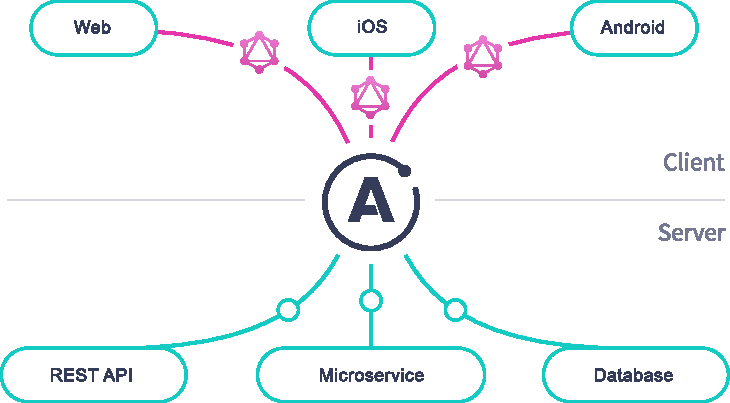
\includegraphics[scale=0.8]{obrazky-figures/apollo_server_diagram}
	\caption{Diagram architektúry Apollo Server. \cite{Apollo}}
\end{figure}

\noindent Apollo Server dokáže pôsobiť ako \emph{jednotná brána} pre všetky klientské aplikácie. Brána má predom definovanú schému, tzn. že klient presne vie aké operácie môže vykonávať a aké dáta môže očakávať späť.

% Slack API
\section{Slack API}
\label{theory:slack_api}
Služba pre tímovú a pracovnú komunikáciu Slack umožňuje vývojárom vytvoriť vlastné aplikácie (Slack apps). Tieto aplikácie následne môžu vykonávať rôzne akcie v~pracovných prostrediach, v~ktorých sú nainštalované. Vo svojej podstate je Slack aplikácia iba HTTP server komunikujúci s~verejným API služby Slack. Vždy, keď užívateľ v aplikácii vykoná nejakú akciu, Slack API upozorní HTTP server danej aplikácie, ktorý akciu spracuje a vyhodnotí (napr. otvorí dialógové okno). \\

\noindent Aplikácie môžu vykonávať niektoré akcie bežných užívateľov \cite{SlackAPI}:

\begin{itemize}
	\item \emph{Odosielať správy} do rôznych koverzácií.
	\item \emph{Čítať správy a konverzácie}.
	\item \emph{Vytvoriť, archivovať a spravovať konverzácie}.
	\item \emph{Reagovať na označenia} od užívateľov.
\end{itemize}

\ldots no verejná API aplikáciam umožňuje aj akcie mimo uživateľských práv \cite{SlackAPI}:

\begin{itemize}
	\item \emph{Otvoriť dialógové okná} pre získanie alebo zobrazenie extra informácií.
	\item \emph{Zostaviť interaktívne komponenty} na ktoré môzu reagovať.
	\item \emph{Vytvoriť a aktualizovať \uv{Home tab} (domovskú obrazovku)} kde môže užívateľ interagovať s~aplikáciou.
	\item \emph{Definovať skratky} vďaka ktorým užívateľ môže rýchlo vykonať akcie v~aplikácii.
\end{itemize}

\subsection{Block Kit}
Framework pre tvorbu užívateľského rozhrania v~Slack aplikáciách, ktorý ponúka kompromis kontroly a flexibility pri budovaní rozhraní v~správach. \cite{SlackAPI}

Užívateľské rozhranie v~Slack aplikácii sa skladá z~blokov rôznych typov vo forme JSON objektov usporiadaných do lineárneho zoznamu. \\

\begin{lstlisting}[caption=Príklad jednoduchého bloku v~Slack aplikácii.]
	{
		"type": "section",
		"text": {
			"type": "mrkdwn",
			"text": "Hello, *World*!"
		}
	},
\end{lstlisting}

\medskip

\noindent Spolu s~blokmi sú v~tejto správe aj metadáta, pomocou ktorých API vie ako má so správou naložiť. Hlavným parametrom metadát je \emph{type}, ktorý môže nadobudnúť jednu z~dvoch hodnôt:

\begin{itemize}
	\item \texttt{home} -- Špecifikuje, že rozhranie má byť použité pre domovskú obrazovku (app\_home).
	\item \texttt{modal} -- Špecifikuje, že rozhranie má byť použité pre dialógové okno.
\end{itemize}

\noindent Lineárny zoznam s~blokmi užívateľského rozhrania sa vloží do parametru \uv{view} v~HTTP správe odoslanej na verejnú API služby Slack. Niektoré bloky podporujú formátovanie svojho obsahu pomocou modifikovanej verzie jazyka \emph{markdown}.

% Headless CMS
%---------------------------------------------------------------------------
\chapter{Headless CMS}
\label{theory:headless}
Headless CMS sú alternatívou k~štandardným redakčným systémom ako napríklad populárny WordPress\footnote{https://wordpress.com/}. Rozdiel medzi headless a štandardnými redakčnými systémami je, že headless systémy nemajú vlastný frontend pre zobrazovanie obsahu a teda \emph{neriešia samotné zobrazenie obsahu} konzumentom.

Takéto systémy typicky disponujú rozhraním REST\footnote{REST -- Representational State Transfer} alebo GraphQL, ktoré implementuje aj táto práca. Jediným spôsobom ako získať obsah z~redakčného systému je využiť niektoré z~dostupných rozhraní poskytované konkrétnym riešením. Výhodou oproti tradičným redakčným systémom je možnosť získané dáta optimálne zobraziť na rôznych zariadeniach. 

\begin{figure}[h]
	\centering
	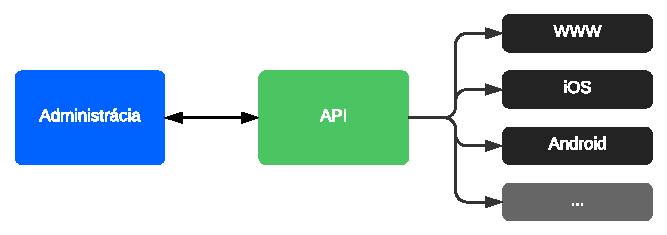
\includegraphics{obrazky-figures/headless_cms_graph.pdf}
	\caption{Ilustračná schéma generického headless redakčného systému.}
\end{figure}

\noindent Členenie obsahu v~takýchto redakčných systémoch je typicky v~dvoch vrstvách -- \emph{kategórie} a \emph{obsahové typy} (komponenty). \\

\noindent \emph{Kategórie} sú zoznamy združujúce jednotlivé komponenty, môžu byť homogénne (všetky prvky zoznamu sú jedného typu) alebo heterogénne (prvky zoznamu sú typicky iných typov). \\

\noindent \emph{Komponenty} sú atomickými prvkami headless redakčných systémov. Môžu nadobúdať rôznych typov, ktoré určujú ich vnútornú dátovú štruktúru. Typický príklad často používaných typov komponentov je napríklad \texttt{prostý text} alebo \texttt{odkaz}. Niektoré headless redakčné systémy umožňujú vytvárať aj vlastné typy komponentov a tak si prospôsobiť dáta vlastným špecifickým potrebám.

% Existujúce riešenia
\section{Existujúce riešenia}
Headless redakčné systémy získavajú na popularite a v~súčasnej dobe existuje množstvo riešení, ktoré sa typicky rozdeľujú do dvoch skupín podľa ukladania a správy dát -- \emph{API-based} a \emph{Git-based}. V~tejto sekcii sú predstavené dva najpopulárnejšie systémy z~každej kategórie.

\subsection{Strapi}
Najpopulárnejší \emph{API-based} headless redakčný systém. Disponuje administračným panelom zostaveným na mieru, REST aj GraphQL rozhraním, systémom uživateľských práv a mnohými inými vlastnosťami. Tento redakčný systém má aj vlastný obchod s~aplikáciami, ktoré si môžu používatelia pridať a tým rozšíriť funkcionalitu. 

\blockquote[Dokumentácia Strapi.io \cite{StrapiDocs}]{Strapi je flexibilný, open-source\footnote{open-source -- otvorený, verejný kód, zväčša vyvíjaný komunitou} headless CMS\footnote{CMS -- ang. content management system (redakčný systém)}, ktorý dáva vývojárom slobodu voľby ich obľúbených nástrojov a zároveň dovoľuje editorom jednoducho spravovať a distribuovať ich obsah.}

\noindent V~prípade, že by užívateľ Strapi redakčného systému mal nakonfigurovanú kolekciu s~názvom \uv{restaurants}, získanie celkového počtu týchto kolekcií v~systéme by mohlo vyzerať takto: \\

\begin{lstlisting}[caption=Príklad HTTP požiadavku na REST rozhranie Strapi.]
	GET "http://localhost:1337/restaurants/count" // Response: 1
\end{lstlisting}

\medskip

\noindent \textbf{Výhody:} Vďaka možnosti definovať vlastné dátové typy je systém flexibilný.

\medskip

\noindent \textbf{Nevýhody:} Pre použitie Strapi je nutné systém spustiť na vlastnej infraštruktúre, pripojiť k~predom vytvorenej relačnej databáze a celý systém nakonfigurovať.

% Netlify CMS
\subsection{Netlify CMS}
Najpopulárnejší \emph{Git-based} headless redakčný systém. Netlify na rozdiel od \emph{API-based} headless redakčných systémov nevyužíva pre ukladanie svojich dát relačnú databázu. Pre uloženie celého obsahu webovej aplikácie využíva repozitáre vytvorené v~prostredí \texttt{git}.

\blockquote[Dokumentácia Netlify CMS \cite{NetlifyDocs}]{Jadro Netlify CMS tvorí React [\ref{theory:react}] aplikácia ktorá využíva rozhranie pre prácu s~GitHub\footnote{\href{https://developer.github.com/v3/}{https://developer.github.com/v3/}}, GitLab\footnote{\href{https://docs.gitlab.com/ee/api/}{https://docs.gitlab.com/ee/api/}} alebo Bitbucket\footnote{\href{https://confluence.atlassian.com/bitbucket/}{https://confluence.atlassian.com/bitbucket/}} API.}

\noindent Netlify sa využíva väčšinou pre menšie stránky ako sú napríklad dokumentácie alebo produktové stránky, pretože umožňuje udržovať obsah relevantný k~danej verzii produktu. \\

\noindent \textbf{Výhody:} Veľmi jednoduchý na používanie, nevyžaduje vlastnú databázu.

\medskip

\noindent \textbf{Nevýhody:} Vhodný len pre statické stránky, obtiažnejšie organizovanie obsahu.

% Návrh riešenia
%---------------------------------------------------------------------------
\chapter{Návrh riešenia}
\label{design}
Kapitola popisuje návrh systému, ktorý je predmetom tejto práce (ďalej ako \uv{\textbf{Slackify}}). Výsledný návrh vznikol po nadobudnutí požadovaných znalostí a analýz požiadaviek kladených na výsledný produkt.

Sekcia \ref{design:assignment} je venovaná konkrétnym funkčným požiadavkám na systém, sekcia \ref{design:use_case} prípadom použitia Slackify v~rôznych scenároch, sekcia \ref{design:architecture} architektúre systému aj s~jej neúspešnými iteráciami. Posledná sekcia \ref{theory:data_types} popisuje špeciálne dátové typy využívané pre uchovávanie a distribúciu dát v~redakčnom systéme Slackify.

% Zadanie práce
\section{Funkčné požiadavky}
\label{design:assignment}
Zadanie, ktorého celé znenie je priložené na \hyperlink{page.2}{strane 2}, popisuje výsledné riešenie práce ako \emph{headless} redakčný systém. Súhrn hlavných požiadaviek na systém je nasledovný:

\begin{itemize}
	\item Užívateľ systému by mal byť schopný spravovať obsah v~\emph{plnej miere} a bez obmedzení v~prostredí služby Slack.
	\item Užívateľ by mal byť schopný začať využívať službu \emph{okamžite} po nainštalovaní do svojho pracovného prostredia v~službe Slack. To znamená, že žiadna konfigurácia alebo nasadenie na vlastnú infraštruktúru by nemalo byť požadované.
	\item Všetky vytvorené dáta by mali byť dostupné cez verejné API.
	\item Systém by mal disponovať webovým rozhraním, odkiaľ by malo byť možné spravovať obsah a nastavenia.
\end{itemize}

\noindent Hlavnou výsadou práce nie je čo najväčšia flexibilita konfigurácie, ale jednoduchosť v~použití a možnosť rýchleho nasadenia. 

\subsection{Odchýlky návrhu od pôvodného zadania}
Slack API umožňuje vytvoriť uživateľské rozhranie zložené z~maximálneho počtu 100 blokov. Pre tento dôvod je maximálny počet zobrazených prvkov v~zoznamoch Slack aplikácie limitovaný. Prvky zoznamov nad určený limit sú skryté a užívateľ ich môže spravovať iba vo webovom prostredí. Nie je teda možné spravovať obsah redakčného systému v~plnej miere za použitia Slack aplikácie ako určuje prvá funkčná požiadavka.

\subsection{Porovnanie s~existujúcimi riešeniami}
Slackify patrí do kategórie \emph{API-driven} headless redakčných systémov. Na rozdiel od iných systémov z~tejto kategórie však Slackify nevyžaduje žiadnu vstupnú konfiguráciu, pretože už disponuje vopred definovanými dátovými typmi, ktoré je možné distribuovať. Redakčný systém je teda možné využívať okamžite, no za cenu menšej flexibility.

% Dátové typy redakčného systému
\section{Dátové typy redakčného systému}
\label{theory:data_types}
Slackify je headless redakčný systém obsahujúci dva hlavné dátové typy -- \emph{collection} (kolekcia) a \emph{component} (komponent). Pomocou týchto dvoch dátových typov je možné vytvoriť logickú štruktúru obsahu, ktorú je možné následne distribuovať pomocou verejného API. Oba dátové typy uchovávajú okrem svojich vlastných parametrov aj momentálny stav uverejnenosti \emph{published}, repretenzovaný dátovým typom \texttt{boolean}.

\subsection{Component}
Component (komponent) je základná dátová struktúra v~Slackify. Celý obsah redakčného systému je zložený z~komponentov usporiadaných do kolekcií [\ref{design:collection}]. Každý komponent má povinnú položku \emph{type} (typ), ktorá určuje ďaľšie zloženie štruktúry.

\subsubsection{Typ \uv{\texttt{Plain Text}}}
Najjednoduchší typ obsahujúci jediné povinné textové pole s~názvom \emph{text}.

\subsubsection{Typ \uv{\texttt{Article}}}
Typ pre vytvorenie jednoduchého článku. Obsahuje povinné textové položky \emph{title} (titulok), \emph{content} (obsah článku) a nepovinnú textovú položku \emph{lead} (úvodný text).

\subsubsection{Typ \uv{\texttt{Link}}}
Typ pre vytvorenie hypertextového odkazu. Obsahuje povinnú textovú položku \emph{url} (cieľová adresa) a voliteľnú textovú položku \emph{text}.

\subsection{Collection}
\label{design:collection}
Collection (kolekcia) je zoznam slúžiaci pre kategorizovanie jednotlivých komponentov. Každá kolekcia ich môže obsahovať 0 až $n$. Jedná sa o~\emph{homogénny zoznam}, tzn. že pri tvorbe kolekcie sa vždy musí zvoliť práve jeden typ komponentov, z~ktorých sa môže zoznam skladať. Každá kolekcia má povinnú položku \emph{name} (názov) a nepovinnú \emph{description} (popis).

% Diagramy prípadov použitia
\section{Diagramy prípadov použitia}
\label{design:use_case}
Diagramy prípadov použitia ukazujú možnosti práce s~redakčným systémom Slakcify z~pohľadu užívateľov s~rôznymi prístupovými oprávneniami (rolami) a zariadenia, ktoré sa snaží získať obsah z~verejného rozhrania.

\subsection{Viewer}
Každému novému užívateľovi, ktorý prepojí svoj účet v~službe Slack so Slackify je automaticky priradená základná užívateľská rola \emph{Viewer}. \\

\noindent Užívateľ s~rolou \emph{Viewer} môže vykonávať nasledujúce akcie:

\begin{itemize}
	\item \texttt{Získať detail kolekcie/komponentu} -- Zobrazenie všetkých informácií o~kolekcii alebo komponente. Dáta je možné iba čítať, nie modifikovať.
	\item \texttt{Získať list kolekcií/komponentov} -- Zobrazenie zoznamu kolekcií alebo komponentov. Komponenty je možné zobraziť všetky alebo podľa pridelených kolekcií. Dáta je možné iba čítať, nie modifikovať.
\end{itemize}

\begin{figure}[H]
	\centering
	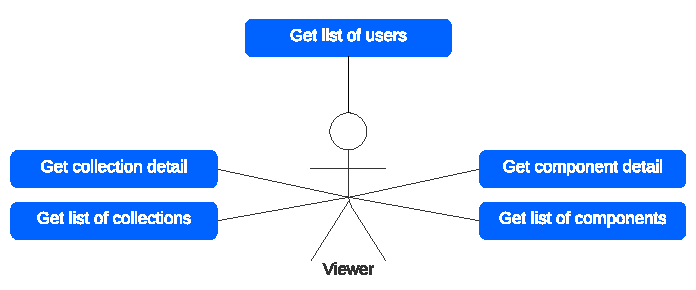
\includegraphics[scale=0.9]{obrazky-figures/viewer_use_case}
	\caption{Diagram prípadov použitia -- \emph{Viewer}.}
\end{figure}

\subsection{Author}
Užívateľská rola \emph{Author} zahŕňa všetky právomoci, ktoré mala rola \emph{Viewer} a rozširuje ich o~možnosť vykonávať nasledujúce akcie:

\begin{itemize}
	\item \texttt{Vytvoriť kolekciu/komponentu} -- Po zadaní a potvrdení vstupných údajov je nová kolekcia alebo komponent pridaná do databázy. Nové komponenty sú inicializované so stavom \emph{hidden} (skrytý, nepublikovaný).
	\item \texttt{Upraviť kolekciu/komponentu} -- Kolekcie alebo komponety je možné upraviť v~ľubovoľný čas. Jediná hodnota, ktorú nie je možné modifikovať je typ kolekcie alebo komponentu.
\end{itemize}

\begin{figure}[H]
	\centering
	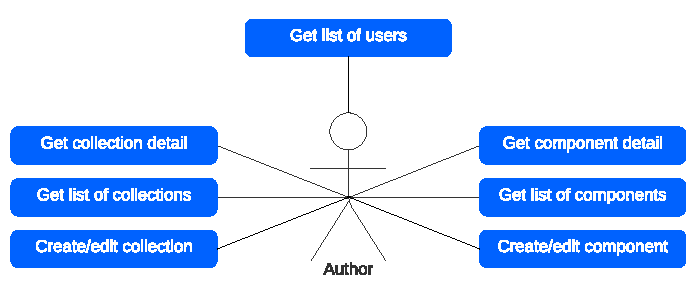
\includegraphics[scale=0.9]{obrazky-figures/author_use_case}
	\caption{Diagram prípadov použitia -- \emph{Author}.}
\end{figure}

\subsection{Editor}
Užívateľská rola \emph{Editor} zahŕňa všetky právomoci, ktoré mala rola \emph{Author} a rozširuje ich o~možnosť vykonávať nasledujúce akcie:

\begin{itemize}
	\item \texttt{Zmazať kolekciu/komponent} -- Kolekcie alebo komponety je možné zmazať v~ľubovoľný čas. Pri zmazaní kolekcie sa zmažú aj všetky komponenty k~nej priradené.
	\item \texttt{Publikovať kolekciu/komponent} -- Publikovaná kolekcia alebo komponent je okamžite dostupná verejne. \emph{Editor} rovnako môže kolekcie alebo komponenty skryť.
\end{itemize}

\begin{figure}[H]
	\centering
	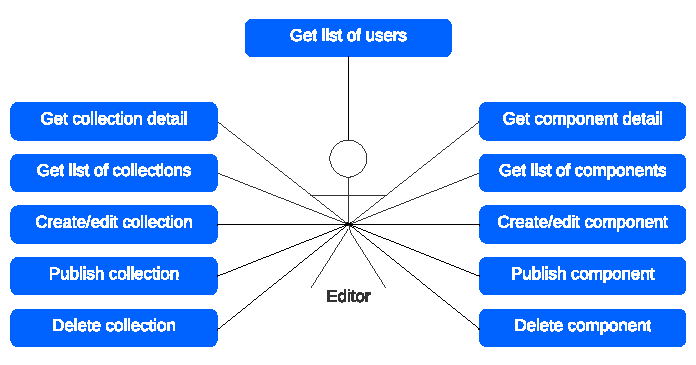
\includegraphics[scale=0.9]{obrazky-figures/editor_use_case}
	\caption{Diagram prípadov použitia -- \emph{Editor}.}
\end{figure}

\subsection{Owner}
Užívateľská rola \emph{Owner} je rola s~najvyššími právomocami. Zahŕňa všetky právomoci, ktoré mala rola \emph{Editor} a rozširuje ich o~možnosť vykonávať nasledujúcu akciu:

\begin{itemize}
	\item \texttt{Zmeniť rolu užívateľa} -- Umožňuje modifikovať užívateľské role ostatných užívateľov. Užívateľ nemôže zmeniť rolu sám sebe. 
\end{itemize}

\begin{figure}[H]
	\centering
	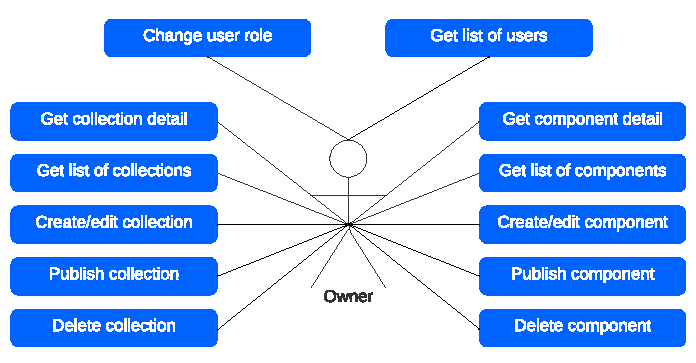
\includegraphics[scale=0.9]{obrazky-figures/owner_use_case}
	\caption{Diagram prípadov použitia -- \emph{Owner}.}
\end{figure}

\subsection{Zariadenie}
Obsah zo Slackify je možné získať z~verejného API prostredníctvom akéhokoľvek zariadenia, ktoré dokáže komunikovať cez protokol HTTP(S). Pre ukážku diagramu prípadov použitia je na mobilnom telefóne nainštalovaná aplikácia, ktorá komunikuje s~rozhraním Slackify. \\

\noindent \emph{Zariadenie} môže v~prostredí Slackify vykonávať nasledujúce akcie:

\begin{itemize}
	\item \texttt{Vyžiadať detail kolekcie/komponentu} -- Informácie o~jednej kolekcií alebo komponente je možné vyžiadať od API pomocou ich unikátneho ID.
	\item \texttt{Vyžiadať list kolekcií} -- Zariadenie si môže vyžiadať zoznam kolekcií. Zoznam kolekcií je v~základnom nastavení zoradený chronologicky podľa času vytvorenia. Výsledky je možné zoradiť alebo filtrovať pomocou parametrov operácie.
	\item \texttt{Vyžiadať list komponentov} -- Pomocou unikátneho ID kolekcie je možné vyžiadať k~nej priradené komponenty. V~prípade neuvedenia ID kolekcie je navrátený list všetkých komponentov v~danom Slack pracovnom prostredí (zoradené chronologicky podľa času vytvorenia). Výsledky je možné zoradiť alebo filtrovať pomocou parametrov operácie.
\end{itemize}

\begin{figure}[H]
	\centering
	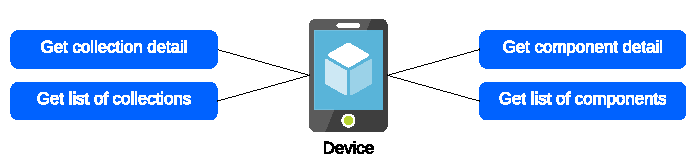
\includegraphics[scale=0.9]{obrazky-figures/device_use_case}
	\caption{Diagram prípadov použitia -- \emph{Zariadenie}.}
\end{figure}

% Návrh architektúry
\section{Návrh architektúry}
\label{design:architecture}
V~počiatočných návrhoch architektúry bol systém rozdelený do dvoch častí:

\begin{itemize}
	\item \texttt{frontend} -- Webová konzola poskytujúca prístup k~obsahu a nastaveniam Slackify.
	\item \texttt{backend} -- Služba zložená z~troch hlavných súčastí:
		\begin{itemize}
			\item[$\circ$] Skryté GraphQL rozhranie poskytujúce prístup k~dátam a logiku pre \texttt{frontend}.
			\item[$\circ$] Verejné GraphQL rozhranie poskytujúce prístup k~obsahu redakčného systému.
			\item[$\circ$] Rozhranie zodpovedné za komunikáciu s verejným API služby Slack.
		\end{itemize}
\end{itemize}

\noindent Neskôr bola však služba \texttt{backend} rozdelená do troch menších samostatných služieb. Finálna architektúra redakčného systému Slackify sa teda skladá z~týchto služieb:

\begin{itemize}
	\item \texttt{frontend} -- Webová konzola poskytujúca prístup k~obsahu a nastaveniam Slackify. Táto časť zostala nezmenená.
	\item \texttt{service-slack} -- Rozhranie zodpovedné za komunikáciu s verejným API služby Slack. Udalosti a akcie prichádzajúce zo Slack aplikácie sú smerované na túto službu, ktorá ich spracuje a vyhodnotí.
	\item \texttt{service-private} -- Skryté GraphQL rozhranie poskytujúce prístup k~dátam a logiku pre \texttt{frontend}.
	\item \texttt{service-public} -- Verejné GraphQL rozhranie poskytujúce prístup k~obsahu redakčného systému.
\end{itemize}

\noindent Takáto architektúra sa oproti jednej veľkej \texttt{backend} službe ukázala ako výhodnejšia z~dvoch hlavných dôvodov. Prvým dôvodom je \emph{jednoduchšia údržba} (napríklad udržovanie logickej súborovej štruktúry bolo pri jednej monolitickej službe obtiažne). Druhým významným dôvodom je možnosť jednotlivé služby \emph{verziovať a vydávať samostatne}, pretože každá služba je nezávislá od ostatných.

\begin{figure}[h]
	\centering
	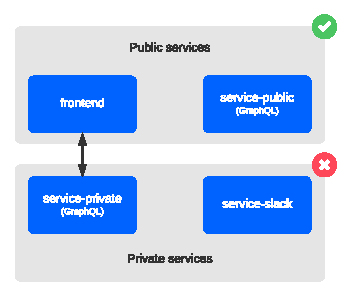
\includegraphics[scale=1.2]{obrazky-figures/architecture}
	\caption{Vizualizácia architektúry podľa návrhu.}
\end{figure}

\noindent Všetky služby využívajú \emph{zdieľanú databázovú vrstvu}, ktorá poskytuje prístup k~dátam uloženým v~relačnej databáze. Celkovo je teda architektúra redakčného systému rozdelená do piatich samostatných súčastí.

% Implementácia
%---------------------------------------------------------------------------
\chapter{Implementácia}
\label{impl}
Ako vysvetľuje sekcia \ref{design:architecture}, headless redakčný systém Slackify je rozdelený do spoločnej databázovej vstvy a štyroch samostatných služieb. Táto kapitola popisuje vybrané časti implementácie všetkých piatich súčastí systému.

Sekcia \ref{impl:database} je venovaná implementácii spoločnej databázovej vrstvy, sekcia \ref{impl:graphql} implementácií verejnej a skrytej GraphQL služby, sekcia \ref{impl:slack_app} implementácii Slack aplikácie. Posledná sekcia \ref{impl:frontend} je venovaná implementácii webovej konzoly.

% Databázová vrstva
\section{Databázová vrstva}
\label{impl:database}
Zdieľaná súčasť systému, ktorá poskytuje prístup k~databáze službám \texttt{service-private}, \texttt{service-public} a \texttt{service-slack}. Pre zostavenie databázy a prístup k~nej je využitá sada nástrojov \texttt{prisma}, bližšie popísaná v~sekcii \ref{theory:databases}.

\subsection{Schéma}
Hlavný konfiguračný súbor sady nástrojov \texttt{prisma}, pomenovaný \texttt{schema.prisma}, ktorý sa skladá z~troch hlavných súčastí:

\begin{itemize}
	\item \texttt{datasource} -- Konfiguračný blok špecifikujúci typ zdroja dát (databázy) a údaje potrebné k~nadviazaniu úspešného pripojenia. Slackify využíva PostgreSQL databázu ako jediný zdroj dát. Environmentálna premenná \texttt{DATABASE\_URL} určuje URL pre pripojenie k~danej databáze (viz výpis \ref{impl:code:prisma_schema}).
	\item \texttt{generator} -- Konfiguračný blok obsahujúci nastavenia automaticky generovaného databázového klienta. Slackify generuje iba jedného databázového klienta do zložky \texttt{node\_modules} v~koreňovom adresári systému. Tento databázový klient je zdieľaný ostatnými službami (viac viz \ref{impl:prisma:client}).
	\item \texttt{model} -- Jednotlivé dátové modely systému, bližšie popísané v~sekcii \ref{impl:data_models}.
\end{itemize}

\noindent Sada nástrojov \texttt{prisma} využíva konfiguračný súbor aj pre \emph{migrácie} databázy. Pri každej zmene dátových modelov automaticky zmení schému databázy a vytvorí nový záznam v~zložke \texttt{migrations}. Tento záznam obsahuje výpis zmien, ktoré migrácia aplikuje, obsah konfiguračného súboru po aplikovaní migrácie a jednotlivé kroky, ktoré migrácia vykoná pre zmenu schémy databázy. Vďaka týmto záznamom je schému databázy možné vrátiť do stavu pred aplikovaním jednej alebo viacerých migrácií.

% TODO: Add language definition for prisma files
\begin{lstlisting}[language={Prisma}, label={impl:code:prisma_schema}, caption=Špecifikácia \texttt{datasource} a \texttt{generator} v~konfiguračnom súbore \texttt{prisma}.]
	datasource db {
		provider = "postgresql"
		url      = env("DATABASE_URL")
		enabled  = env("DATABASE_URL")
	}

	generator cient_common {
		provider = "prisma-client-js"
		output   = "../../node_modules/@prisma/client"
	}
\end{lstlisting}

\subsection{Dátové modely}
\label{impl:data_models}
Dátové modely definované v~konfiguračnom súbore \texttt{prisma} reprezentujú entity využívané v~aplikácii. Sada nástrojov \texttt{prisma} tieto modely automaticky mapuje do jednotlivých tabuliek v~databáze. \\

\noindent Slackify obsahuje dva hlavné modely \texttt{Collection} a \texttt{Component} reprezentujúce obsah uložený v~redakčnom systéme. Ďaľšie modely \texttt{User} a \texttt{Team} slúžia pre uchovávanie informácií o~užívateľoch a tímoch (pracovných prostredí) \emph{prepojených so službou Slack}.

\subsubsection{Model \texttt{Collection}}
Dátový model \texttt{Collection} (kolekcia) slúžiaci ako zoznam pre jednotlivé komponenty. Sú to homogénne zoznamy, ktoré môžu obsahovať iba komponenty jedného typu. \\

\begin{lstlisting}[language={Prisma}, caption=Dátový model \texttt{Collection} v~konfiguračnom súbore \texttt{prisma}.]
	model Collection {
		id          String        @default(cuid()) @id
		name        String
		type        ComponentType
		published   Boolean       @default(false)
		description String?
		team        Team          @relation(...)
		teamId      String
		components  Component[]
		createdAt   DateTime      @default(now())
		updatedAt   DateTime      @updatedAt
	}
\end{lstlisting}

\medskip

\noindent Popis niektorých významných položiek obsiahnutých v~dátovom modeli:

\begin{itemize}
	\item \texttt{type} -- Určuje jediný typ komponentu, ktorý je možné vložiť do danej kolekcie. Typ komponentu je bližšie popísaný v~sekcii \ref{impl:model:component}.
	\item \texttt{team} -- Relácia s~dátovým modelom \texttt{Team} ku ktorému je kolekcia priradená. Každá kolekcia musí byť priradená k~práve jednej entite modelu \texttt{Team}.
	\item \texttt{components} -- Relácia 1~:~$n$ všetkých komponentov priradených ku kolekcii. Každá kolekcia môže mať 0 až $\infty$ priradených komponentov.
\end{itemize}

\subsubsection{Model \texttt{Component}}
\label{impl:model:component}
Dátový model \texttt{Component} (komponent) reprezentujúci malú časť obsahu v~Slackify. Každý komponent \emph{musí mať zvolený typ}, ktorý určuje vnútornú štruktúru dát uložených v~komponente. \\

\begin{lstlisting}[language={Prisma}, caption=Dátový model \texttt{Component} v~konfiguračnom súbore \texttt{prisma}.]
	model Component {
		id              String                  @default(cuid()) @id
		type            ComponentType           @default(PLAIN_TEXT)
		published       Boolean                 @default(false)
		collection      Collection              @relation(...)
		collectionId    String
		author          User                    @relation(...)
		authorId        String
		team            Team                    @relation(...)
		teamId          String
		plainTextDataId String?
		plainTextData   PlainTextComponentData? @relation(...)
		articleDataId   String?
		articleData     ArticleComponentData?   @relation(...)
		linkDataId      String?
		linkData        LinkComponentData?      @relation(...)
		createdAt       DateTime                @default(now())
		updatedAt       DateTime                @updatedAt
	}
\end{lstlisting}

\medskip

\noindent Popis niektorých významných položiek obsiahnutých v~dátovom modeli:

\begin{itemize}
	\item \texttt{type} -- Typ komponentu nadobúdajúci jednu z~hodnôt výčtového typu \texttt{ComponentType}.
	\item \texttt{collection} -- Relácia s~dátovým modelom \texttt{Collection}. Každý komponent musí byť priradený k~práve jednej kolekcii.
	\item \texttt{author} -- Relácia s~dátovým modelom \texttt{Author}. Každý komponent musí byť priradený k~právej jednému autorovi.
	\item \texttt{team} -- Relácia s~dátovým modelom \texttt{Team}. Každý komponent musí byť priradený k~práve jednému tímu.
\end{itemize}

\noindent Hodnota položky \texttt{type} určuje práve jednu z~položiek \texttt{plainTextData}, \texttt{articleData} alebo \texttt{linkData} ako povinnú. Tieto položky ukazujú na rôzne špecifické dátové modely, ktoré reprezentujú obsah daných komponentov. Napríklad ak položka \texttt{type} má hodnotu \texttt{LINK}, položka \texttt{linkData} \emph{musí} byť reláciou na dátový model \texttt{LinkComponentData}, ktorý obsahuje povinné pole URL a nepovinné pole text. \\

\begin{lstlisting}[language={Prisma}, caption=Dátový model \texttt{LinkComponentData} v~konfiguračnom súbore \texttt{prisma}.]
	model LinkComponentData {
		id   String  @default(cuid()) @id
		text String?
		url  String
	}
\end{lstlisting}

\subsubsection{Výčtový typ \texttt{ComponentType}}
Výčtový typ (enum), ktorý môže nadobúdať jednu z~hodnôt \texttt{PLAIN\_TEXT}, \texttt{ARTICLE} alebo \texttt{LINK}. \\

\begin{lstlisting}[language={Prisma}, caption=Výčtový typ \texttt{ComponentType} v~konfiguračnom súbore \texttt{prisma}.]
	enum ComponentType {
		PLAIN_TEXT
		ARTICLE
		LINK
	}
\end{lstlisting}

\subsubsection{Model \texttt{User}}
Dátový model \texttt{User} (užívateľ) reprezentujúci informácie o~užívateľskom účte prepojenom so službou Slack. \\

\begin{lstlisting}[language={Prisma}, caption=Dátový model \texttt{User} v~konfiguračnom súbore \texttt{prisma}.]
	model User {
		id          String      @id
		email       String      @unique
		name        String
		role        UserRole    @default(VIEWER)
		accessToken String      @unique
		image_24    String?
		image_32    String?
		image_48    String?
		image_72    String?
		image_192   String?
		image_512   String?
		team        Team        @relation(fields: [teamId], references: [id])
		teamId      String
		components  Component[]
	}
\end{lstlisting}

\medskip

\noindent Popis niektorých významných položiek obsiahnutých v~dátovom modeli:

\begin{itemize}
	\item \texttt{id} -- Jedinečný identifikátor užívateľa, prevzatý z~autentifikačnej API služby Slack.
	\item \texttt{role} -- Užívateľská rola nadobúdajúca jednu z~hodnôt výčtového typu \texttt{UserRole}. Určuje právomoci užívateľa, inicializuje sa s~hodnotou \texttt{VIEWER}.
	\item \texttt{team} -- Relácia s~dátovým modelom \texttt{Team}. Každý užívateľ musí byť priradený k~práve jednému tímu.
	\item \texttt{components} -- Relácia 1~:~$n$ všetkých komponentov, ktorých je užívateľ autorom. Každý užívateľ môže byť autorom 0 až $\infty$ komponentov.
\end{itemize}

\subsubsection{Výčtový typ \texttt{UserRole}}
Výčtový typ (enum), ktorý môže nadobúdať jednu z~hodnôt \texttt{VIEWER}, \texttt{AUTHOR}, \texttt{EDITOR} alebo \texttt{OWNER}. \\

\begin{lstlisting}[language={Prisma}, caption=Výčtový typ \texttt{UserRole} v~konfiguračnom súbore \texttt{prisma}.]
	enum UserRole {
		OWNER
		EDITOR
		AUTHOR
		VIEWER
	}
\end{lstlisting}

\subsubsection{Model \texttt{Team}}
Dátový model \texttt{Team} (tím) reprezentujúci informácie o~tíme (pracovnom prostredí, workspace) v~službe Slack. \\

\begin{lstlisting}[language={Prisma}, caption=Dátový model \texttt{Team} v~konfiguračnom súbore \texttt{prisma}.]
	model Team {
		id          String       @id
		name        String
		domain      String       @unique
		accessToken String       @unique
		collections Collection[]
		users       User[]
		components  Component[]
	}
\end{lstlisting}

\medskip

\noindent Popis niektorých významných položiek obsiahnutých v~dátovom modeli:

\begin{itemize}
	\item \texttt{id} -- Jedinečný identifikátor tímu, prevzatý z~autentifikačnej API služby Slack.
	\item \texttt{accessToken} -- Generovaný prístupový kód, ktorý je nutné využiť pre získanie obsahu z~redakčného systému cez verejné API (službu \texttt{service-public}). 
	\item \texttt{collections} -- Relácia 1~:~$n$ všetkých kolekcií, ktoré sú vytvorené pod daným tímom. Každý tím môže mať priradených 0 až $\infty$ kolekcií.
	\item \texttt{users} -- Relácia 1~:~$n$ všetkých užívateľov, ktorí sú členmi daného tímu. Každý tím môže mať 0 až $\infty$ užívateľov.
	\item \texttt{components} -- Relácia 1~:~$n$ všetkých komponentov, ktoré sú vytvorené pod daným tímom. Každý tím môže mať priradených 0 až $\infty$ komponentov.
\end{itemize}

\subsection{Automaticky generovaný databázový klient}
\label{impl:prisma:client}
Pomocou konfiguračného súboru \texttt{prisma} automaticky zostrojí striktne typovaného databázové klienta, ktorý dokáže zostavovať dotazy pre databázu. Pomocou tohto klienta je možné vytvárať, čítať, modifikovať, či mazať dáta v~databáze. \\

\noindent Databázový klient je generovaný do zložky \texttt{node\_modules}, odkiaľ je možné ho importovať ako z~modulu \texttt{@prisma/client}. \\

\begin{lstlisting}[caption=Príklad vytvorenia inštancie databázového klienta v~Slackify.]
	import { PrismaClient } from "@prisma/client";

	export const prisma = new PrismaClient();
\end{lstlisting}

% GraphQL služby
\section{GraphQL služby}
\label{impl:graphql}
Ako bolo vysvetlené v~sekcii \ref{design:architecture} o~návrhu architektúry, redakčný systém Slackify disponuje dvomi GraphQL službami -- skrytou \texttt{service-private} a verejnou \texttt{service-public}. Obe GraphQL služby sú implementované pomocou balíčka Apollo Server.

\subsection{Schéma}
GraphQL schémy oboch služieb sú implementované pomocou balíčka \texttt{Nexus Schema}, ktorý umožňuje vytvoriť GraphQL schému v~jazyku JavaScript namiesto SDL\footnote{SDL -- Schema Definition Language} definovanom v~GraphQL špecifikácii. Vďaka tomu je možné budovať schému \uv{code-first} a silno typovanú. \\

\begin{lstlisting}[caption=Časť GraphQL schémy služby \texttt{service-private}., label={impl:code:schema}]
	export const Query = queryType({
		definition(t) {
			/* Users */
			t.crud.users({
				filtering: {
					team: true,
				},
			});
		}
	});
\end{lstlisting}

\noindent Balíček \texttt{Nexus Schema} disponuje aj pluginom, ktorý ho dokáže prepojiť s~\texttt{prisma} klientom. Toto prepojenie rozširuje triedu \texttt{t} (prvý parameter v~bloku \texttt{definition()}) o~dve položky:

\begin{itemize}
	\item \texttt{t.model} -- Mapovanie položiek databázových modelov na GraphQL typy.
	\item \texttt{t.crud} -- Databázové operácie automaticky generované pre každý databázový model. Operácie podporujú stránkovanie, filtrovanie alebo zoraďovanie výsledkov. Vo výpise \ref{impl:code:schema} je znázornená operácia na získanie listu všetkých užívateľov s~možnosťou filtrácie podľa tímu.
\end{itemize}

\noindent Plugin pre prepojenie schémy s~\texttt{prisma} klientom však nepodporuje kontrolu autorizácie užívateľa, tá je riešená použitím \uv{middleware} funkcií.

\subsection{Autorizácia}
Každá požiadavka a mutácia (s~výnimkou mutácie \texttt{signIn()} služby \texttt{service-private}) musí obsahovať HTTP hlavičku s~názvom \texttt{Authorization}. Obe GraphQL služby však vyžadujú rozdielne hodnoty tejto hlavičky, bližšie popísané v~sekciách \ref{impl:service-private} a \ref{impl:service-public}.

\subsubsection{GraphQL Shield}
Skrytá aj verejná GraphQL služba pre kontrolu prístupu využíva aj middleware \texttt{GraphQL Shield}, ktorý umožňuje vytvoriť \uv{pravidlá} pre prístup ku konkrétnym požiadavkám alebo mutáciám. \\

\begin{lstlisting}[caption={Pravidlo \texttt{GraphQL Shield} kontrolujúce či je užívateľ autentifikovaný.}, label={impl:code:rule}]
	export const isAuthenticated = rule({ cache: 'contextual' })(
		async (_parent, _args, { user }: Context) => {
			return user !== undefined;
		}
	);
\end{lstlisting}

\medskip

\noindent Podobné pravidlá ako vo výpise \ref{impl:code:rule} sú využité pre kontrolu prístupu v~celej GraphQL schéme. Ak niektorá z~podmienok pravidla nie je splnená, dané pravidlo obvykle vráti inštanciu typu \texttt{Error} so špecifickou správou, ktorá je zaslaná späť do webovej konzoly. Ak sú však splnené \emph{všetky podmienky}, pravidlo vracia boolean hodnotu \texttt{true} a riadenie je prenechané príslušnej GraphQL \texttt{resolver} funkcii.

\subsection{Skrytá služba \texttt{service-private}}
\label{impl:service-private}
Skrytá GraphQL služba (\texttt{service-private}) poskytuje prístup k~dátam pre webové konzolu (službu \texttt{frontend}, ktorej implementácia je popísaná v~sekcii \ref{impl:frontend}). Schéma tejto služby je tvorená prevažne CRUD operáciami nad databázovými modelmi \texttt{Collection} a \texttt{Component}.

\subsubsection{Autorizácia}
HTTP hlavička \texttt{Authorization} požiadavky alebo mutácie obsahuje JWT\footnote{JWT -- JSON Web Token} konkrétneho užívateľa. Tento token obsahuje okrem iných informácií o~užívateľovi aj jeho ID. Vďaka tomu je možné pred vykonaním každej operácie získať všetky dostupné informácie o~užívateľovi a jeho tíme, ktoré sú následne dostupné v~kontexte každej GraphQL \texttt{resolver} funkcie. Ak nebolo možné nájsť užívateľa s~daným ID, dáta o~ňom a jeho tíme majú v~GraphQL \texttt{resolver} funkcii hodnotu \texttt{undefined}.

\subsection{Verejná služba \texttt{service-public}}
\label{impl:service-public}
Verejná GraphQL služba (\texttt{service-public}) slúži ako hlavné aplikačné rozhranie pre headless redakčný systém Slackify. Tento GraphQL server umožňuje vývojárom využívajúcim Slackify vo svojich implementáciach jednoducho získať obsah z~redakčného systému.

\subsubsection{Autorizácia}
Po prepojení tímu v~službe Slack s~redakčným systémom Slackify je tomuto tímu vygenerovaný \emph{unikátny autorizačný token}. Tento token je následne očakávaný v~HTTP hlavičke \texttt{Authorization} každej požiadavky smerujúcej na službu \texttt{service-public}. V~prípade, že autorizačný token chýba alebo je nesprávny, služba požiadavku zahodí a odpovie chybovou správou vysvetľujúcou zlyhanie. 

\subsubsection{Zjednodušený typ \texttt{Component}}
Databázový model \texttt{Component} slúži pre uchovávanie metadát o~komponente. Samotný obsah komponentu sa nachádza v~oddelených databázových modeloch s~ktorými je komponent v~relácií (viac viz \ref{impl:model:component}). Takýto princíp ukladania dát umožňuje jednoduchú modifikáciu typov komponentov a ich obsahu, no nie je optimálny pre vývojárov, ktorí využívajú Slackify vo svojich projektoch. \\

\begin{lstlisting}[language={GraphQL}, caption={Príklad získania obsahu komponentu pred optimalizáciou.}]
	query {
		component(...) {
			id
			type # ?? - Unknown type
			plainTextData
			articleData
			linkData
			...
		}
	}
\end{lstlisting}

\medskip

\noindent Vývojár musí totiž vopred poznať typ komponentu a podľa toho si vyžiadať z~GraphQL servera konkrétnu reláciu s~obsahom komponentu. Väčši problém však nastane v~prípade, že vývojár vopred nepozná typ komponentu, ktorý žiada od GraphQL servera. V~takejto situácií je nutné vyžiadať relácie s~obsahmi pre \emph{všetky typy komponentov} a po obdržaní dát pristúpiť k~správnemu obsahu podľa typu. \\

\begin{lstlisting}[caption={Definícia union typu pre dáta komponentu.}, label={impl:service-public:union}]
	export const ComponentData = unionType({
		name: 'ComponentData',
		definition(t) {
			t.members('PlainTextComponentData', 'ArticleComponentData', 'LinkComponentData');
			t.resolveType((data) => {
				// ...
			});
		},
	});
\end{lstlisting}

\medskip

\noindent Z~tohto dôvodu dôvodu služba \texttt{service-public} disponuje upraveným typom \texttt{Component}, ktorý má špeciálne pole \texttt{data} typu \texttt{union} (viz výpis \ref{impl:service-public:union}). Toto pole združuje relácie s~obsahom pre všetky typy komponentov. Ak si vývojár vyžiada toto pole, získa obsah komponentu bez ohľadu na to, akého je typu.

\subsubsection{Zber štatistík}
Verejná GraphQL služba zaznamenáva jednoduché štatistiky prístupu k~obsahu jednotlivých komponentov. Vždy, keď je nejaký komponent vyžiadaný z~tohto rozhrania služba vytvorí nový záznam v~databáze. Záznam sa skladá z~času a ID komponentu a je vytvorený aj keď je komponent obsiahnutý ako súčasť požiadavky na kolekciu.

% Webová konzola
\section{Webová konzola}
\label{impl:frontend}
Webová konzola (služba \texttt{frontend}) slúži pre komplexnejšiu správu obsahu v~Slackify redakčnom systéme. Samotné uživateľské rozhranie je implementované pomocou JavaScriptovej knižnice React a frameworku Next.js, ktorý zabezpečuje vykresľovanie (render) na strane servera.

\subsection{Pridanie Slackify do pracovného prostredia}
Pred prvým použítím Slackify je nutné redakčný systém (konkrétne jeho Slack aplikáciu) pridať do pracovného prostredia pomocou OAuth 2.0\footnote{\href{https://oauth.net/2/}{https://oauth.net/2/}} brány služby Slack.  \\

\noindent Proces pridania Slackify do pracovného prostredia je nasledovný:

\begin{enumerate}
	\item Užívateľ, ktorý chce pridať Slackify do svojho pracovného prostredia je po kliknutí na tlačidlo \uv{Add to Slack} presmerovaný na autorizačnú stránku Slacku.
	\item Po úspešnej autorizácií aplikácie je užívateľ presmerovaný späť na stránku vo webovej konzole Slackify \texttt{/auth/add} s~URL parametrom \textit{code} (dočasný prístupový kód).
	\item Slackify vymení obsah parametra \textit{code} za informácie o~danom pracovnom prostredí a užívateľovi, ktorý aplikáciu do pracovného prostredia pridal.
	\item Informácie o~pracovnom prostredí sú pridané do databázy spolu s~užívateľom, ktorý má automaticky priradenú rolu \emph{Owner}.
\end{enumerate}

\noindent Slackify je možné pridať do pracovného prostredia aj v~obchode s~aplikáciami v~Slacku. 

\subsection{Prihlásenie užívateľa}
Slackify nemá vlastný proces vytvorenia užívateľského účtu, naopak všetky \emph{dáta o~užívateľoch preberá z~služby Slack} pomocou OAuth 2.0 brány služby Slack. \\

\noindent Proces príhlásenia užívateľa do Slackify je nasledovný:

\begin{enumerate}
	\item Užívateľ, ktorý sa chce prihlásiť do Slackify je po kliknutí na tlačidlo \uv{Sign in with Slack} presmerovaný na autorizačnú stránku služby Slack.
	\item Užívateľ vyplní svoje prihlasovacie údaje pre účet v~tom pracovnom prostredí, \emph{ktoré má nainštalovanú aplikáciu Slackify}.
	\item Po úspešnom prihlásení užívateľ \emph{povolí Slackify prístup k~užívateľským údajom} a je následne presmerovaný na stránku vo webovej konzole Slackify \texttt{/auth/redirect} s~URL parametrom \textit{code}.
	\item Slackify odošle hodnotu URL parametra \textit{code} na OAuth API služby Slack a očakáva odpoveď s~\emph{autorizačným kódom pre daného užívateľa} a informáciach o~ňom.
	\item Autorizačný token je následne možné využiť pre opätovné získanie informácií o~užívateľovi alebo k~vykonávaniu akcií za užívateľa.
\end{enumerate}

\noindent Po úspešnom obdržaní autorizačného tokena a užívateľských dát systém skontroluje, či už daný užívateľ v~databáze existuje. V~prípade, že užívateľ neexistuje, je záznam o~ňom pridaný do databázy. V~prípade, že už existuje, informácie o~ňom sú len aktualizované. \\

\noindent Vygenerovaný JWT so základnými informáciami o~užívateľovi je uložený do cookies prehliadača. Pri návšteve každej stránky prebieha kontrola, či uložený JWT nie je expirovaný.

\subsection{Správa kolekcií}
Hlavnou súčasťou správy kolekcií je zoznam všetkých kolekcií, ktoré boli vytvorené v~tíme aktuálne prihláseného užívateľa. Na tejto stránke je možné kolekcie vytvoriť, upraviť alebo zmazať, ak má užívateľ na tieto akcie dostatočné práva.

\begin{figure}[h]
	\centering
	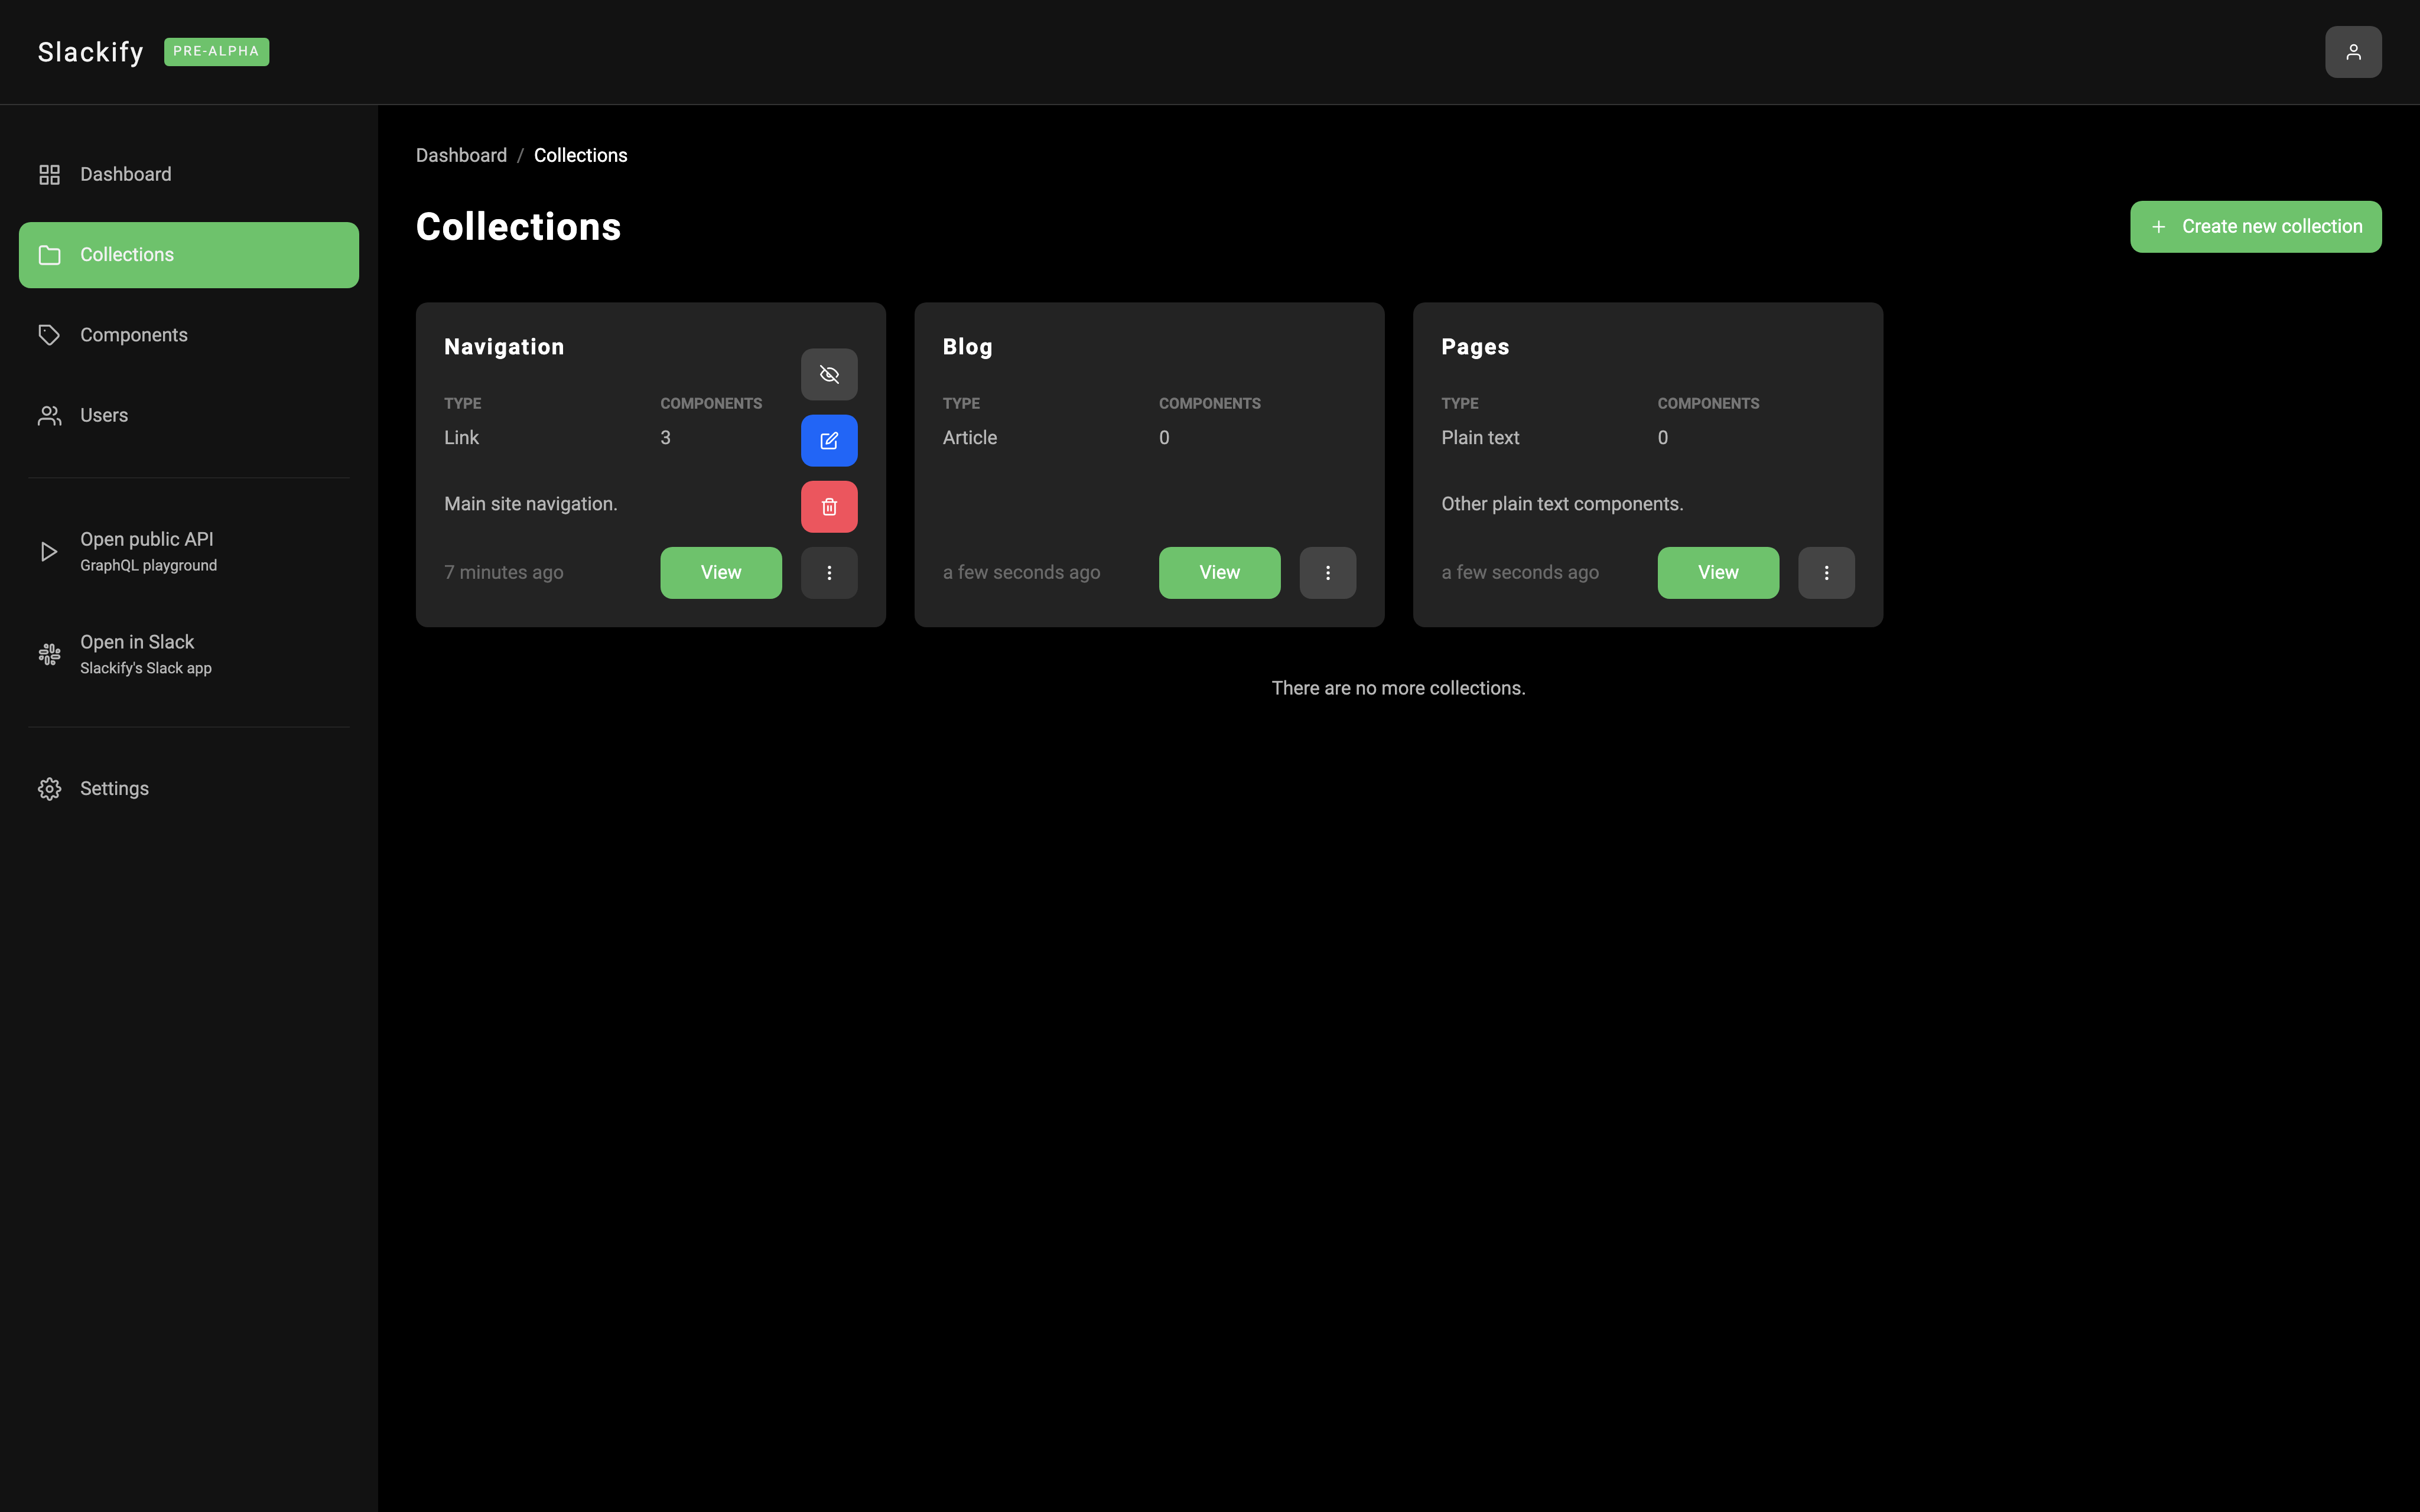
\includegraphics[scale=0.085]{obrazky-figures/screenshot_collections}
	\caption{Stránka správy kolekcií vo webovej konzole.}
\end{figure}

\noindent Pri úvodnom načítaní stránky je odoslaná GraphQL požiadavka (query) \texttt{collections()}, ktorá získa prvých 40 kolekcií zo služby \texttt{service-private}. Ak chce užívateľ zobraziť viac kolekcií, musí zísť na koniec zoznamu. Na jeho konci sa nachádza element, ktorý ak je viditeľný v~okne prehliadača odošle znova požiadavku \texttt{collections()}, ale tentoraz s~priloženými parametrami \texttt{skip} a \texttt{first}. Získané položky sú pridané na koniec zoznamu a takto je vytvorený mechanizmus tzv. \uv{nekonečného scrollovania} (infinite scrolling).

\subsubsection{Vytvorenie a úprava kolekcie}
Vytvorenie novej kolekcie alebo úprava už existujúcej je možná pomocou dialógového okna, ktoré je dostupné na stránkach zoznamu a detailu kolekcií. Objekt uložený v~globálnom stave aplikácie pod názvom \texttt{createUpdateModal} uchováva kontext dialógového okna, ktorý obsahuje položky:

\begin{itemize}
	\item \texttt{mode} -- Mód zobrazenia, môže nadobudnúť hodnoty \uv{create} alebo \uv{update}.
	\item \texttt{collection} -- V~prípade, že mód zobrazenia má hodnotu \uv{update}, očakáva sa, že hodnota tejto položky obsahuje objekt popisujúci upravovanú kolekciu.
\end{itemize}

\noindent Po potvrdení formulára vytvorenia alebo úpravy kolekcie je na službu \texttt{service-private} odoslaná mutácia \texttt{createOneCollection()}, resp. \texttt{updateOneCollection()} s~dátami z~formulára. Ak bola mutácia úspešná, v~odpovedi od služby \texttt{service-private} by sa mali nachádzať dáta novej, resp. aktualizovanej kolekcie. Tieto dáta sú následne použité pre aktualizovanie cache webovej aplikácie.

\begin{figure}[H]
	\centering
	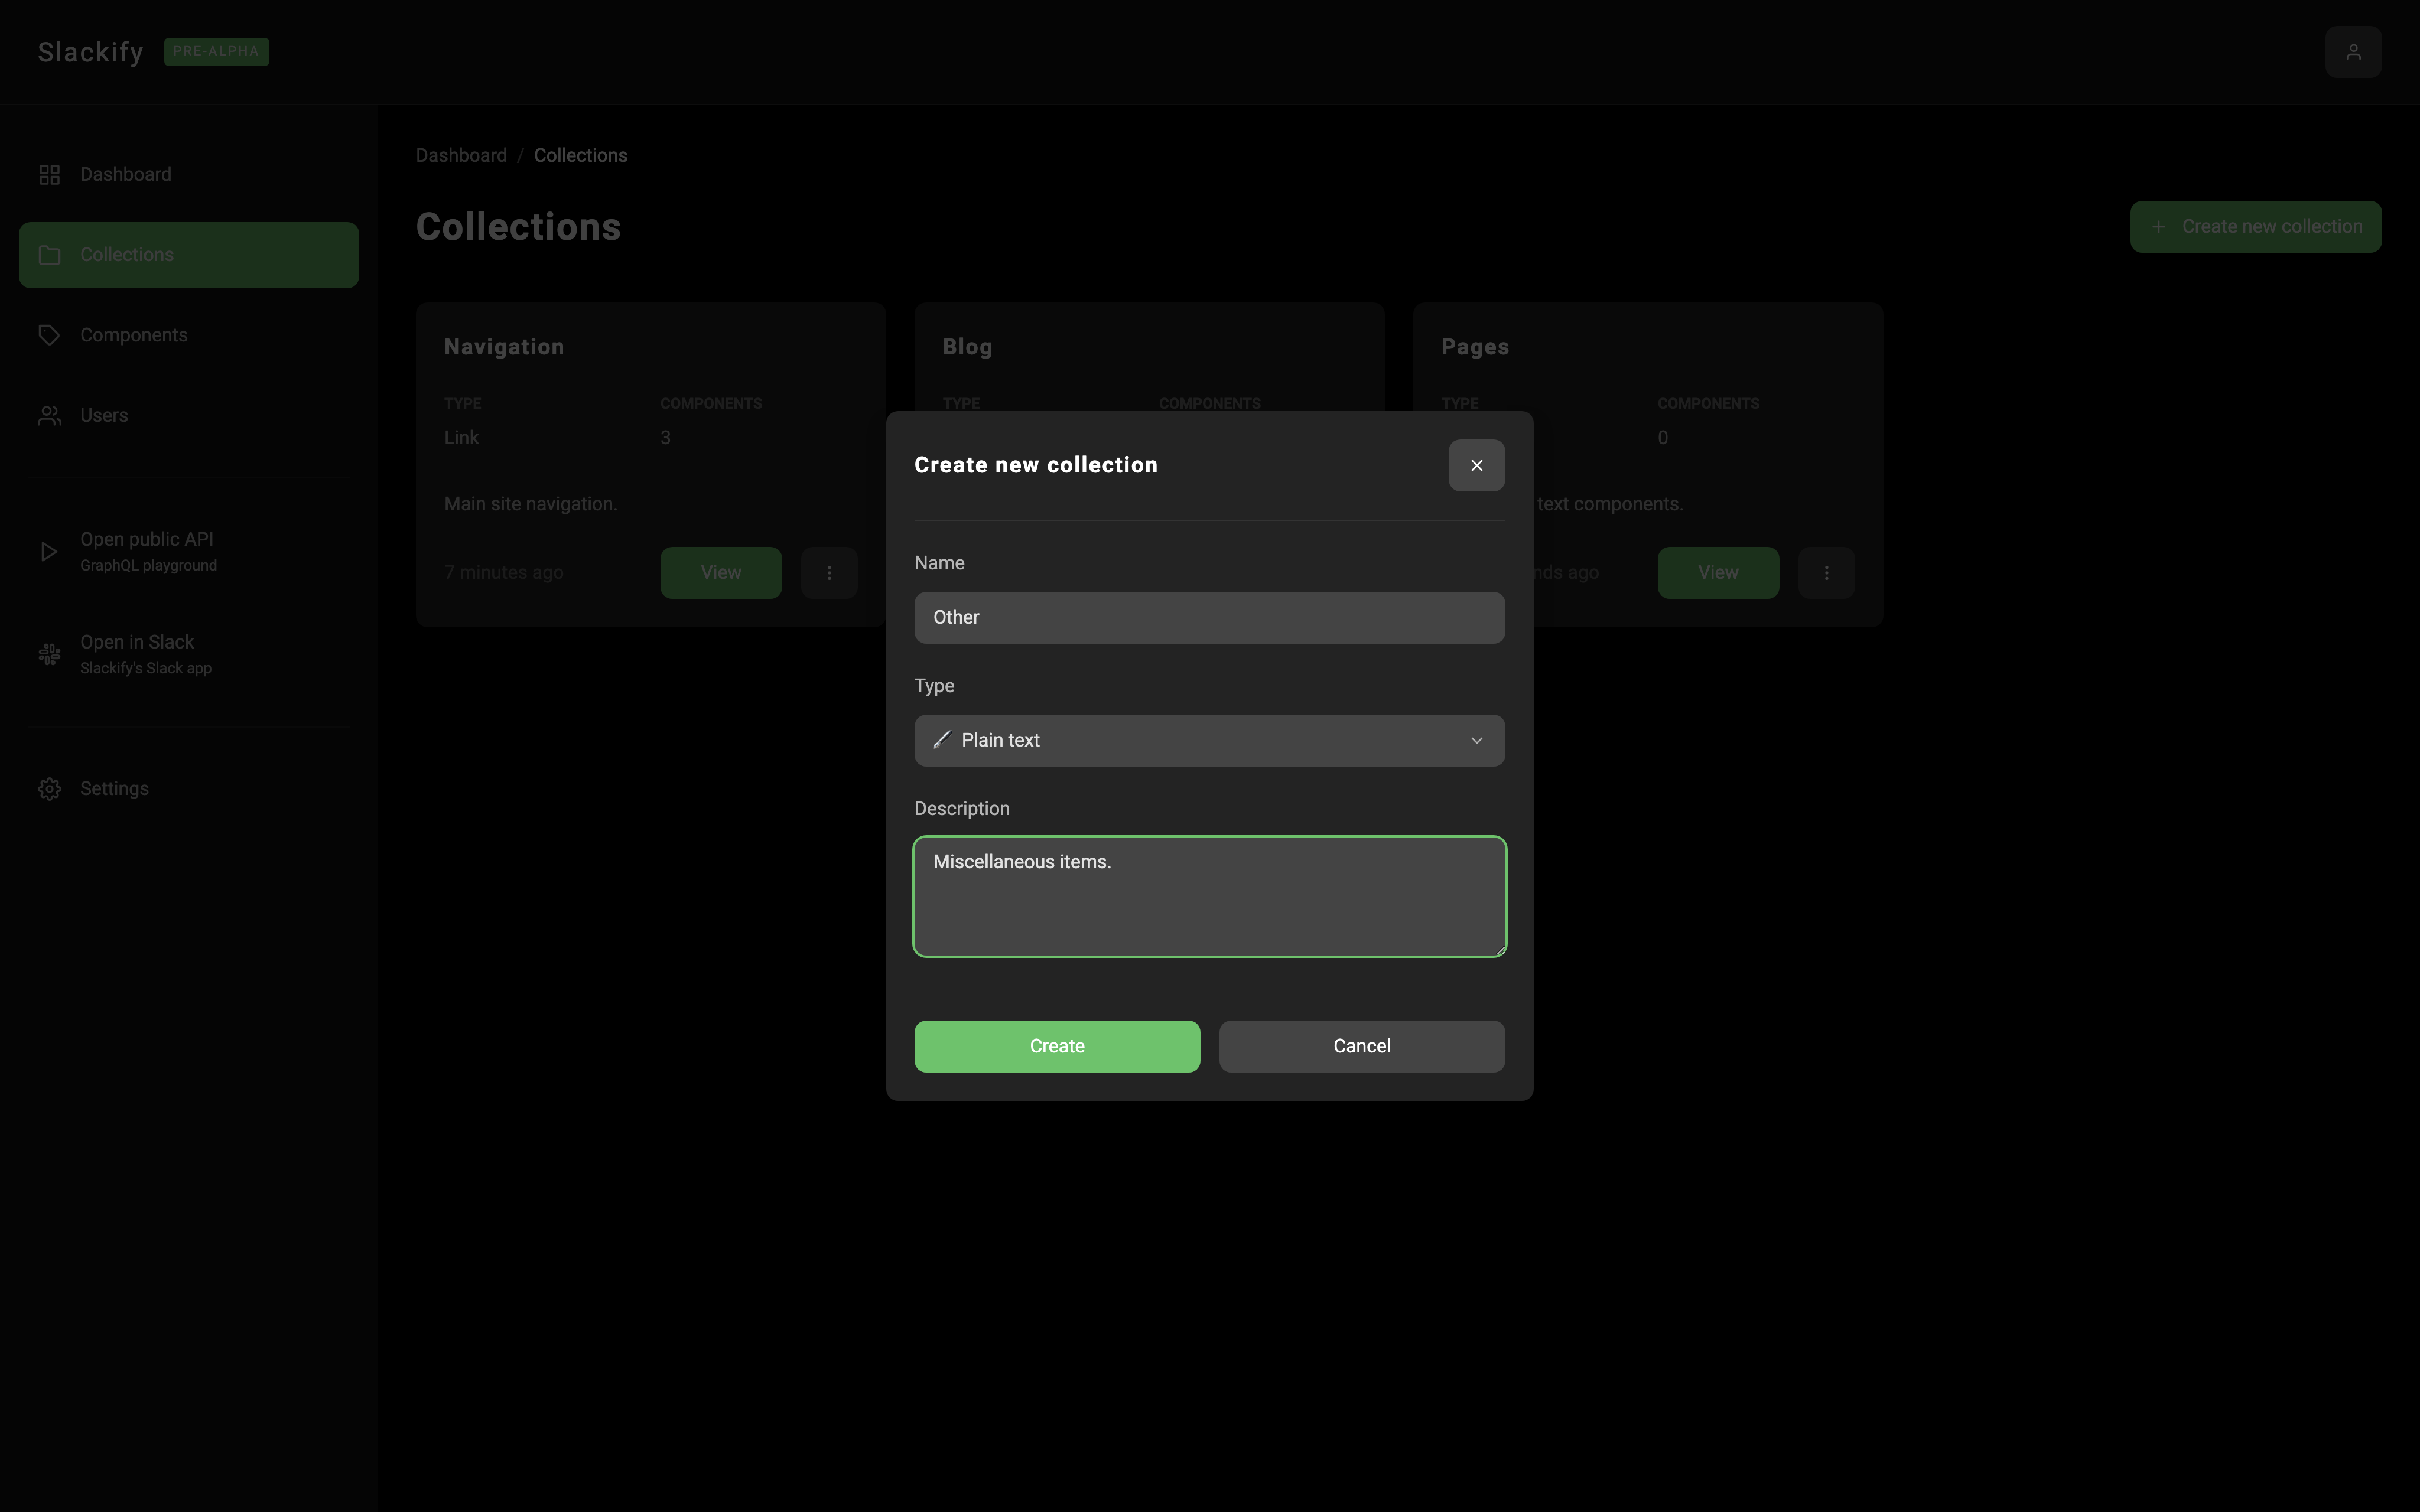
\includegraphics[scale=0.085]{obrazky-figures/screenshot_collection_create}
	\caption{Dialógové okno pre vytvorenie a úpravu kolekcií.}
\end{figure}

\subsection{Správa komponentov}
Podobne ako u~kolekcií je hlavnou súčasťou správy komponentov zoznam všetkých komponentov, ktoré boli vytvorené v~tíme aktuálne prihláseného užívateľa. Podmienkou vytvorenia nového komponentu je už \emph{aspoň jedna existujúca kolekcia}, ku ktorej môže byť daný komponent priradený. Na tejto stránke je možné okrem vytvorenia nového komponentu aj upraviť alebo zmazať už existujúce komponenty.

\begin{figure}[H]
	\centering
	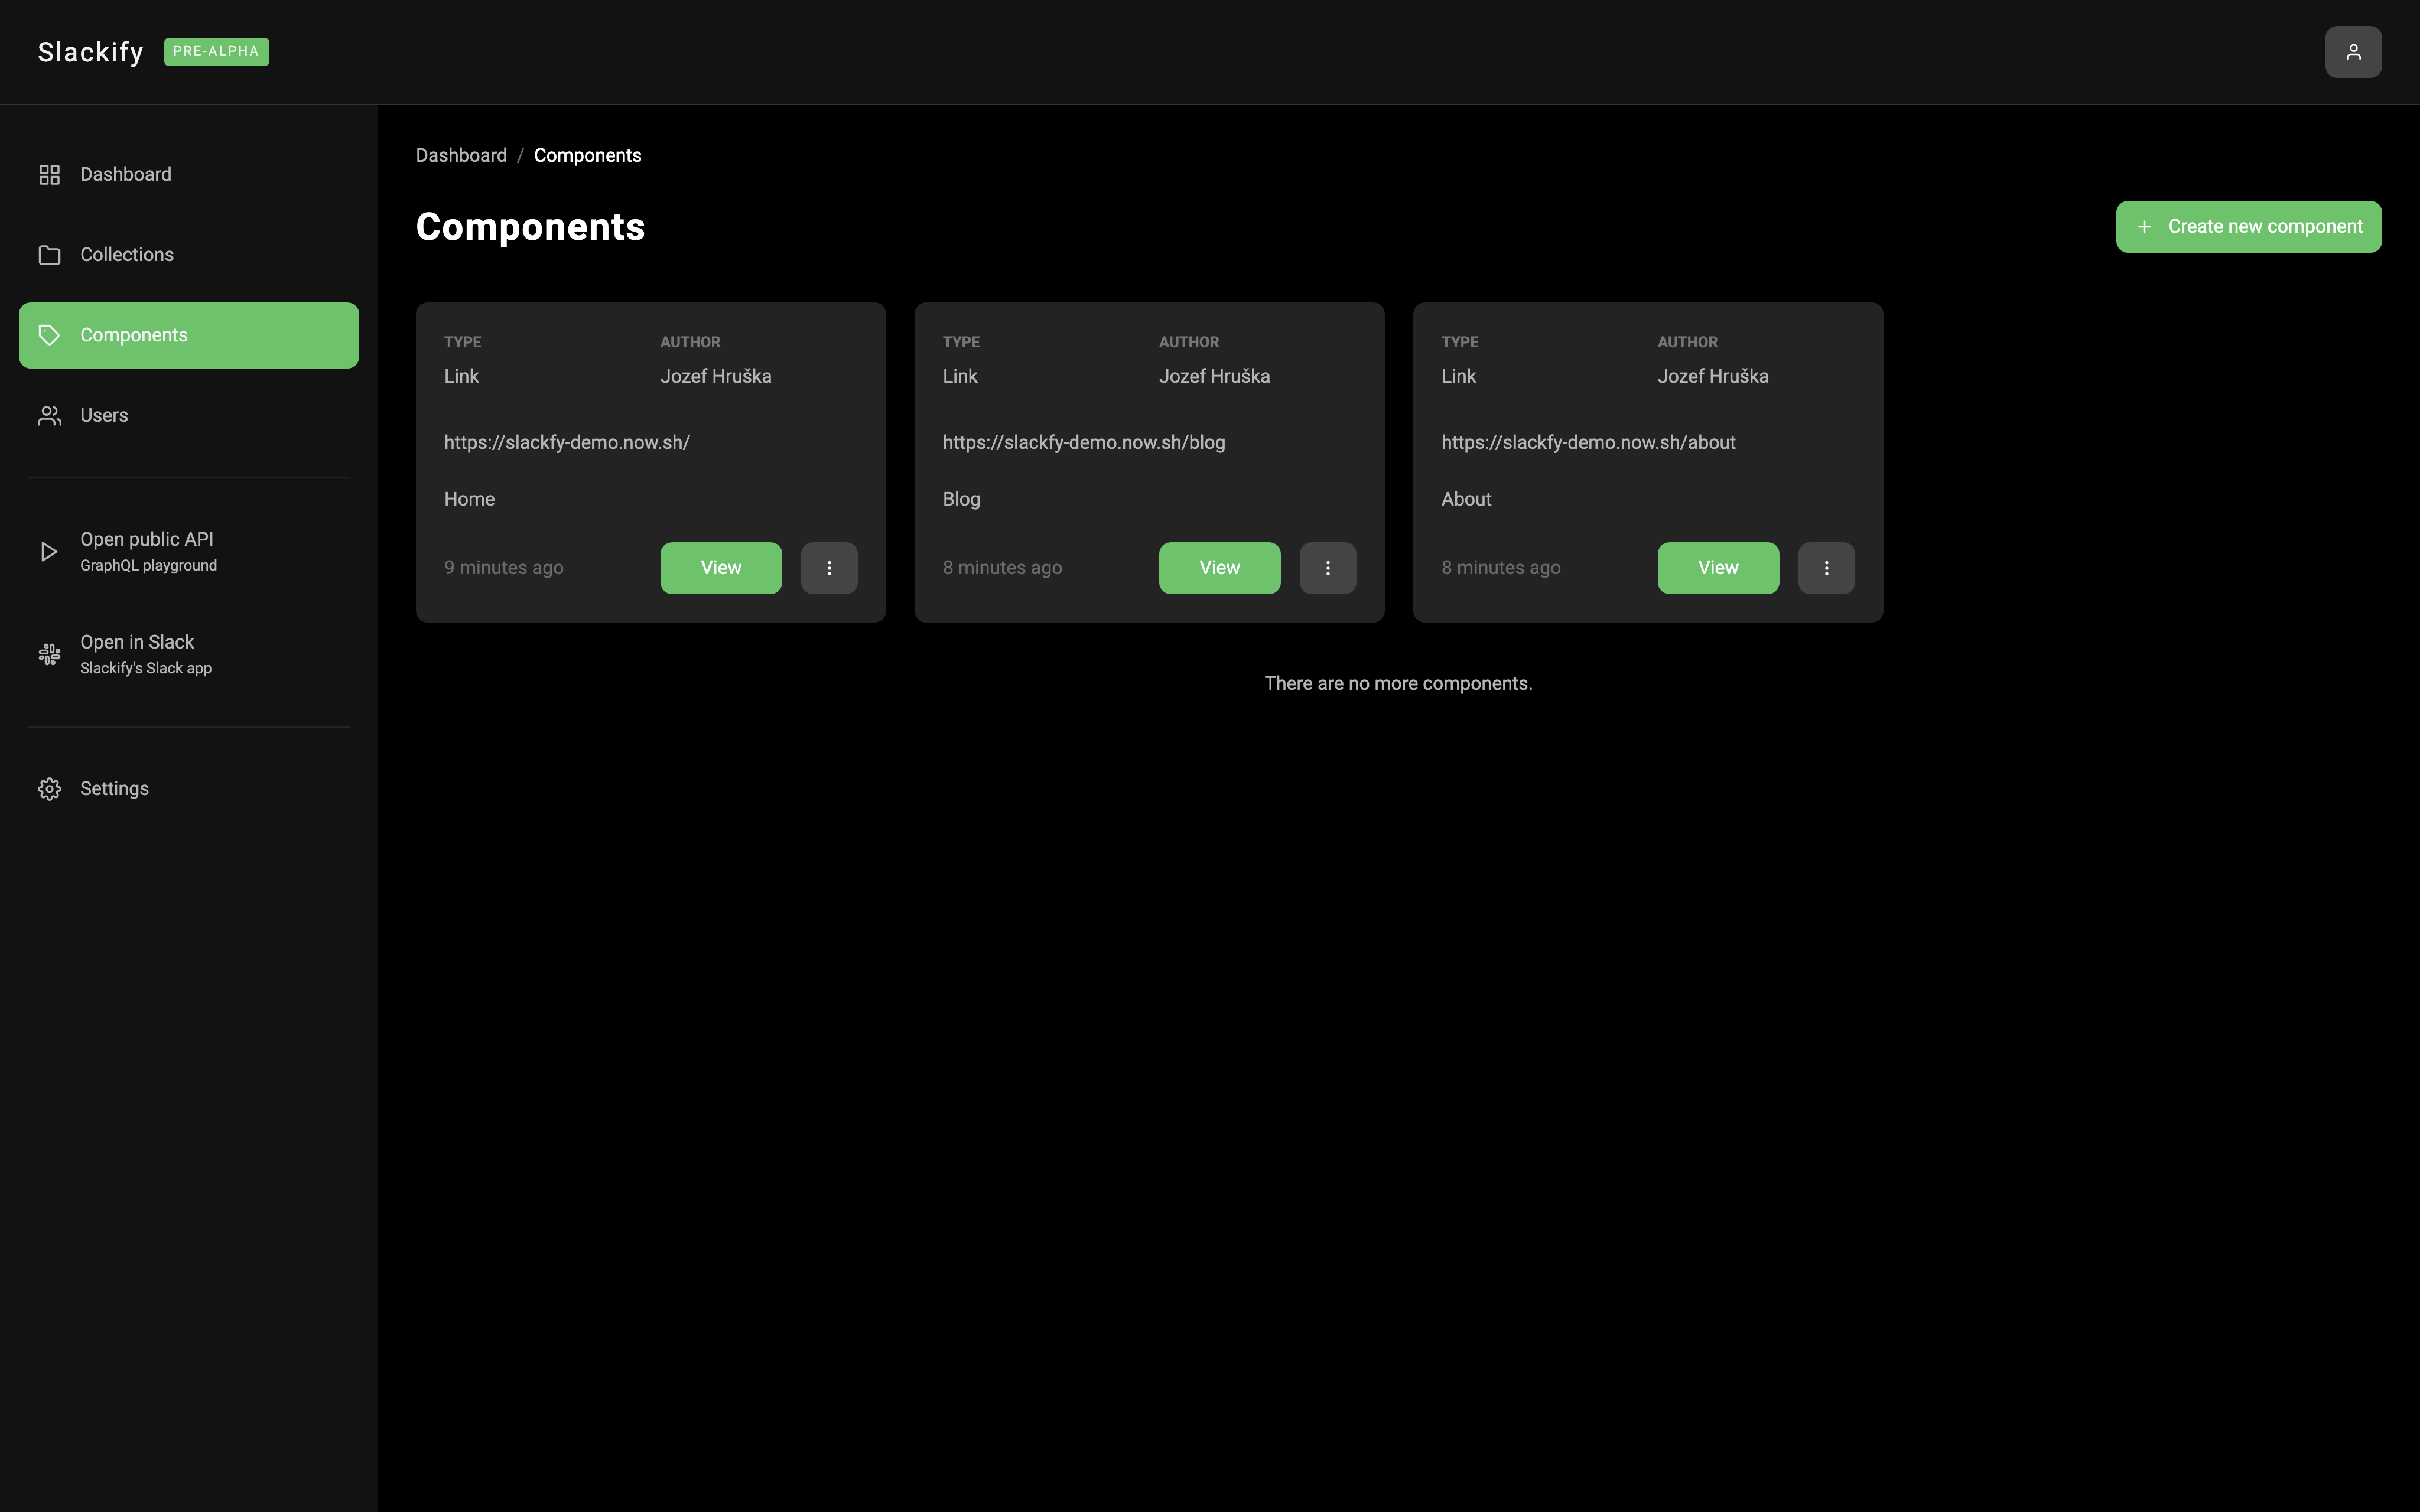
\includegraphics[scale=0.085]{obrazky-figures/screenshot_components}
	\caption{Stránka správy komponentov vo webovej konzole.}
\end{figure}

\noindent Rovnako ako pri zozname kolekcií je pri úvodnom načítaní odoslaná požiadavka pre získanie komponentov, z~ktorých sa zoznam zostaví. Pre komponenty je táto požiadavka pomenovaná \texttt{components()}. Zoznam komponentov takisto podporuje aj infinite scrolling mechanizmus.

\subsubsection{Vytvorenie a úprava komponentov}
Rovnaký princíp ako pri tvorbe a úprave kolekcií. Jedná sa o~dialógové okno, ktoré svoj kontext uchováva v~globálnom stave aplikácie, avšak mierne pozmenený:

\begin{itemize}
	\item \texttt{mode} -- Mód zobrazenia, rovnako ako u~kolekcií môže nadobudnúť hodnoty \uv{create} alebo \uv{update}.
	\item \texttt{collection} -- Obsahuje informácie o~aktuálne zvolenej kolekcii pri tvorbe nového komponentu. Typ kolekcie určuje typ k~\emph{nej priradených komponentov}, a preto je táto kolekcia využitá pre zobrazenie relevantného formulára pre konkrétny typ komponentov.
	\item \texttt{component} -- V~prípade, že mód zobrazenia má hodnotu \uv{update}, očakáva sa, že hodnota tejto položky obsahuje objekt popisujúci upravovaný komponent.
\end{itemize}

\begin{figure}[H]
	\centering
	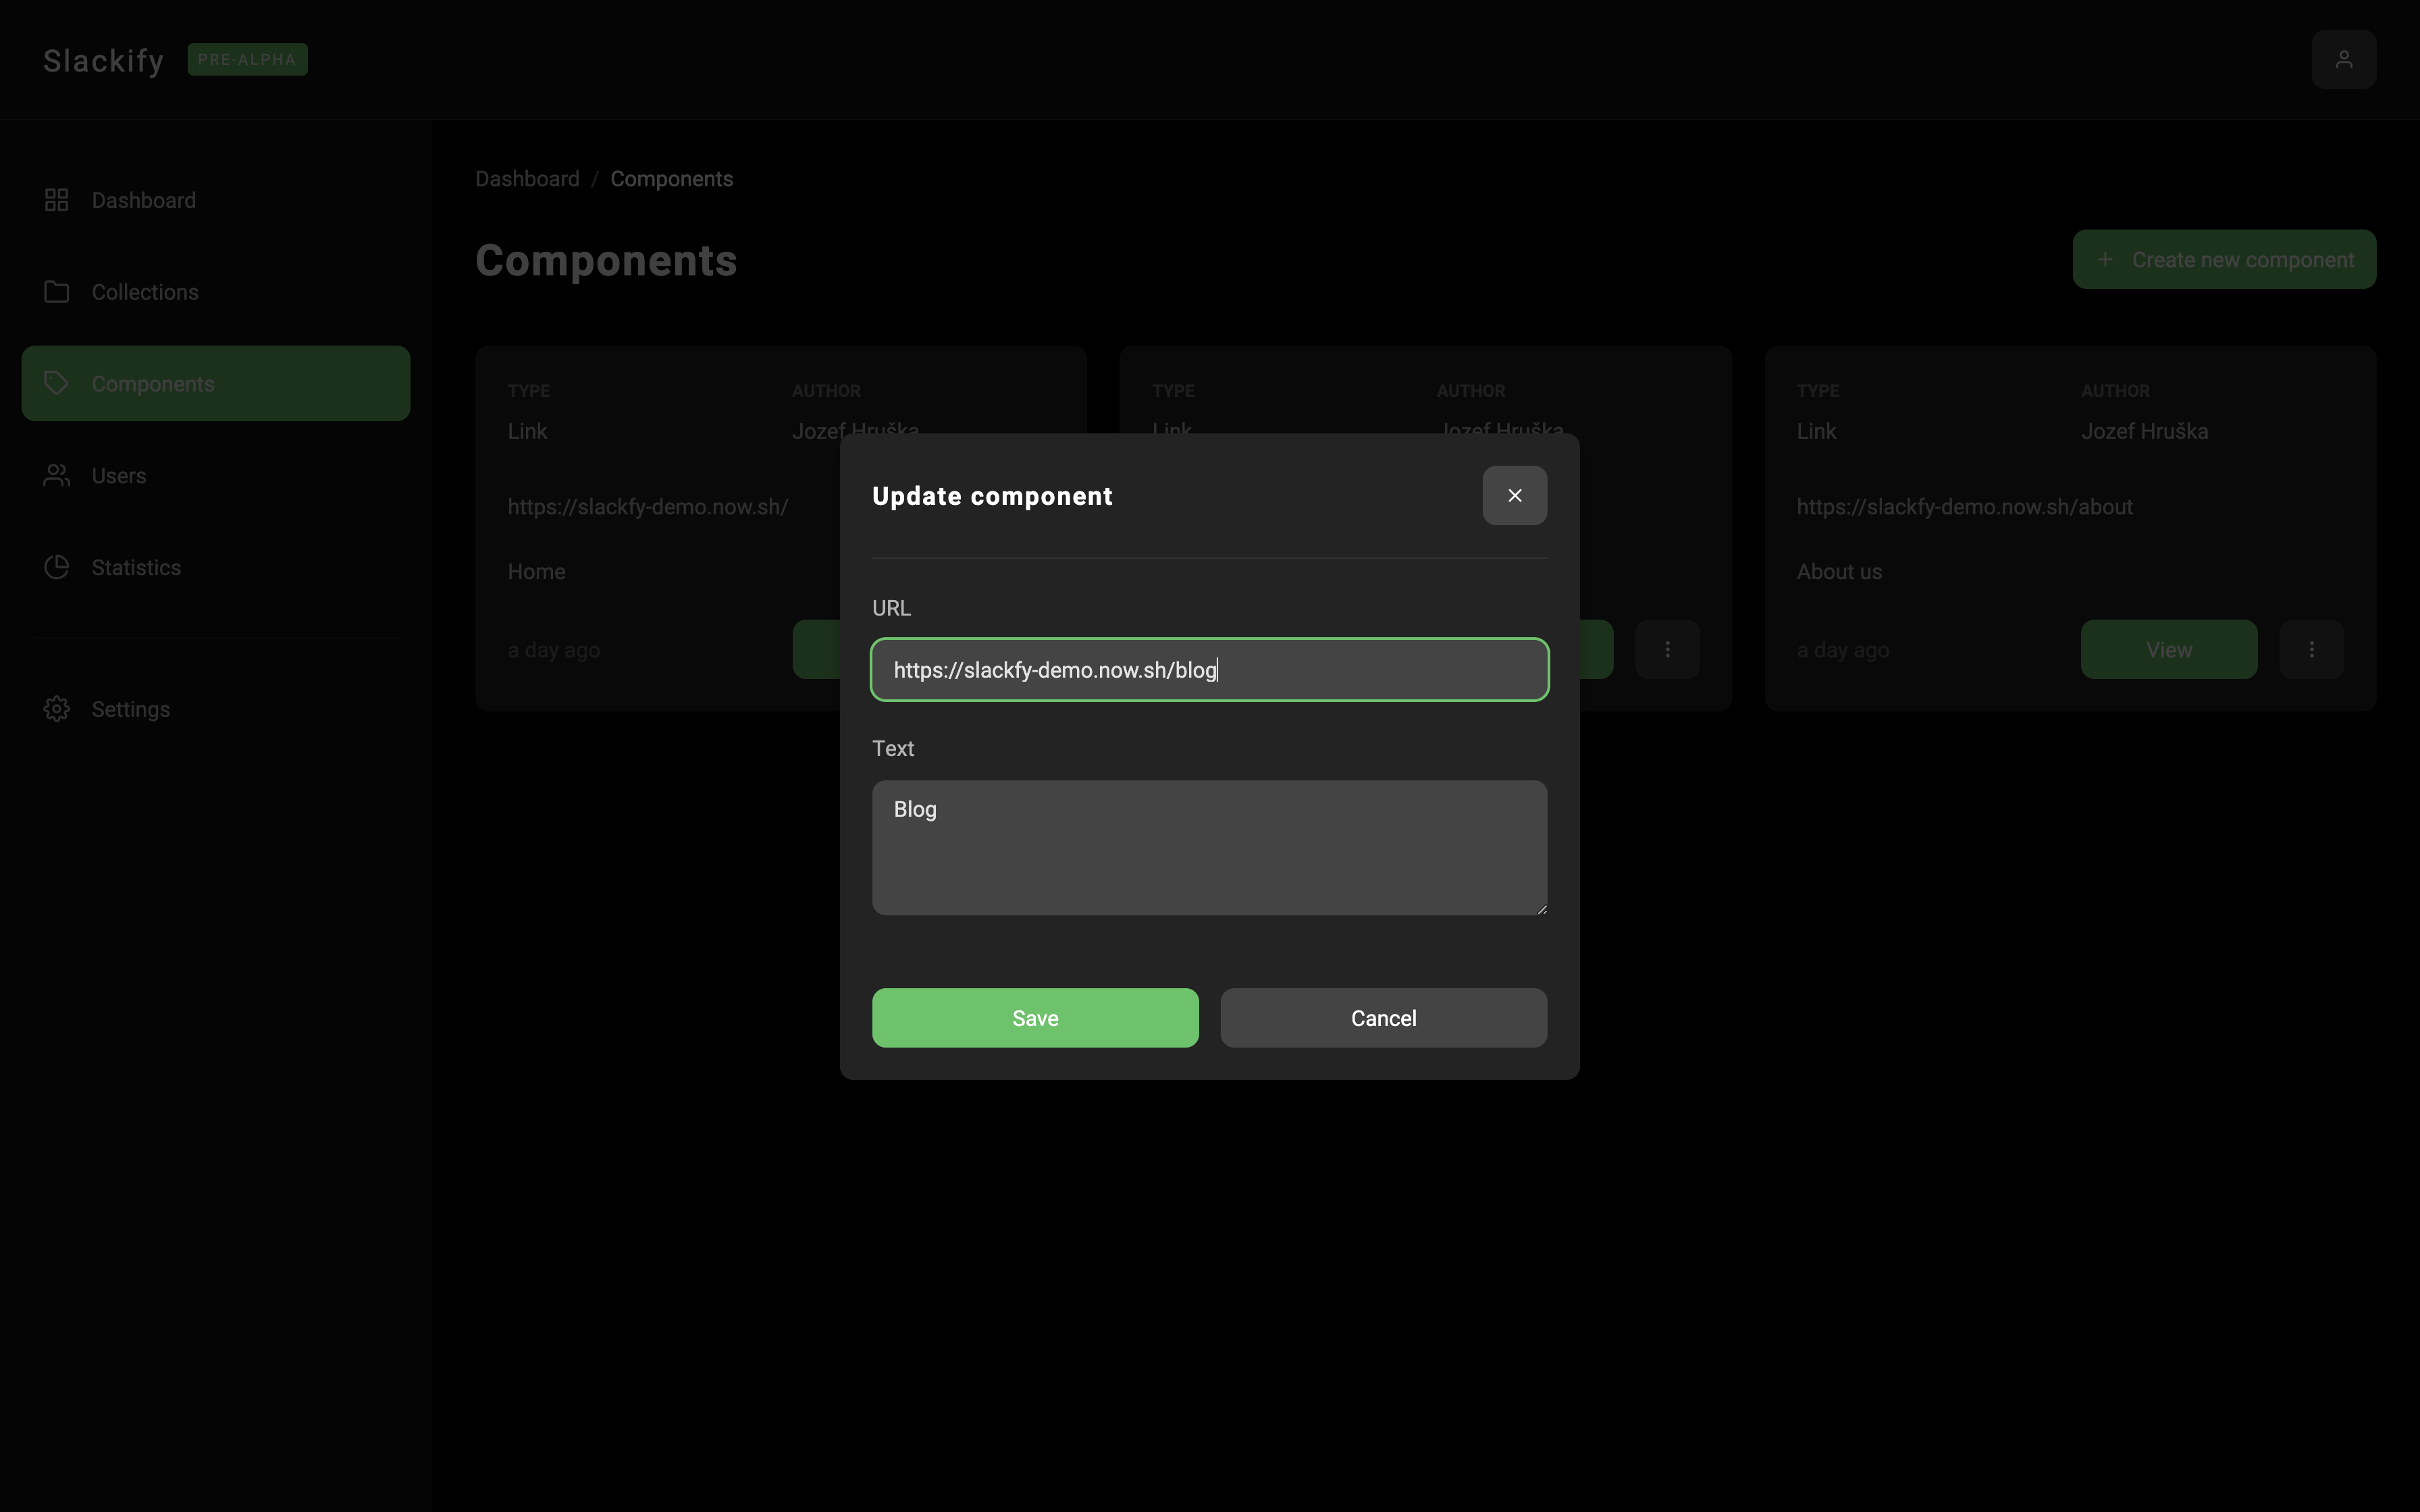
\includegraphics[scale=0.085]{obrazky-figures/screenshot_component_update}
	\caption{Dialógové okno pre vytvorenie a úpravu komponentov.}
\end{figure}

\noindent Po povrdení formulára je pre vytvorenie nového komponentu alebo úpravu už existujúceho odoslaná mutácia \texttt{createOneComponent()}, resp. \texttt{updateOneComponent()} na službu \texttt{service-private}.

\subsection{Zmena role užívateľa}
Každý užívateľ môže navštíviť stránku so zoznamom všetkých užívateľov tímu, ktorého je členom. V~prípade, že má aktuálne prihlásený užívateľ rolu \uv{Owner}, môže navyše meniť role ostatných užívateľov v~rámci tímu. U~každého užívateľa v~zozname sa nachádza HTML element \texttt{<Select />}, ktorý ukazuje aktuálnu rolu daného užívateľa. Pri zmene na inú hodnotu tento element odošle mutáciu \texttt{updateOneUser()} so zvolenou hodnotou na službu \texttt{service-private}, ktorá aktualizuje rolu daného užívateľa.

% Slack aplikácia
\section{Slack aplikácia}
\label{impl:slack_app}
Služba \texttt{service-slack} je Slack aplikácia umožňujúca \emph{plnohodnotnú správu obsahu} v~redakčnom systéme Slackify. Jedná sa o~HTTP server implementovaný pomocu balíčka Bolt od spoločnosti Slack, ktorý reaguje na udalosti (events) a akcie (actions) prichádzajúce z verejnej API služby Slack.

\subsection{Autorizácia tímov}
Slack aplikácia sa musí pri každej akcii autorizovať špeciálnym tokenom \uv{bot token} unikátnym pre každý tím (pracovné prostredie) prepojený s aplikáciou. Na túto autorizáciu slúži metóda \texttt{authorize()}, ktorá vyhľadá \uv{bot token} konkrétneho tímu podľa jeho ID, ktoré je obsiahnuté v každej prichádzajúcej akcii alebo udalosti.

\subsection{Domovská stránka}
Každá Slack aplikácia má k~dispozícií jednu stránku, ktorej obsah môže prispôsobiť danému užívateľovi. Táto stránka má názov \uv{App Home} a v~Slackify slúži ako jediné miesto, kde môže užívateľ spravovať obsah redakčného systému. Pri každej návšteve tejto stránky užívateľom Slack API odošle udalosť \texttt{app\_home\_opened} na službu \texttt{slackify-slack}. Po obrdžaní udalosti služba vygeneruje rohranie pre daného užvateľa a odošle ho späť na Slack API, ktoré sa postará aby bolo správne zobrazené užívateľovi v~aplikácii. Rozhranie domovskej stránky je \emph{perzistentné}.

\begin{figure}[h]
	\centering
	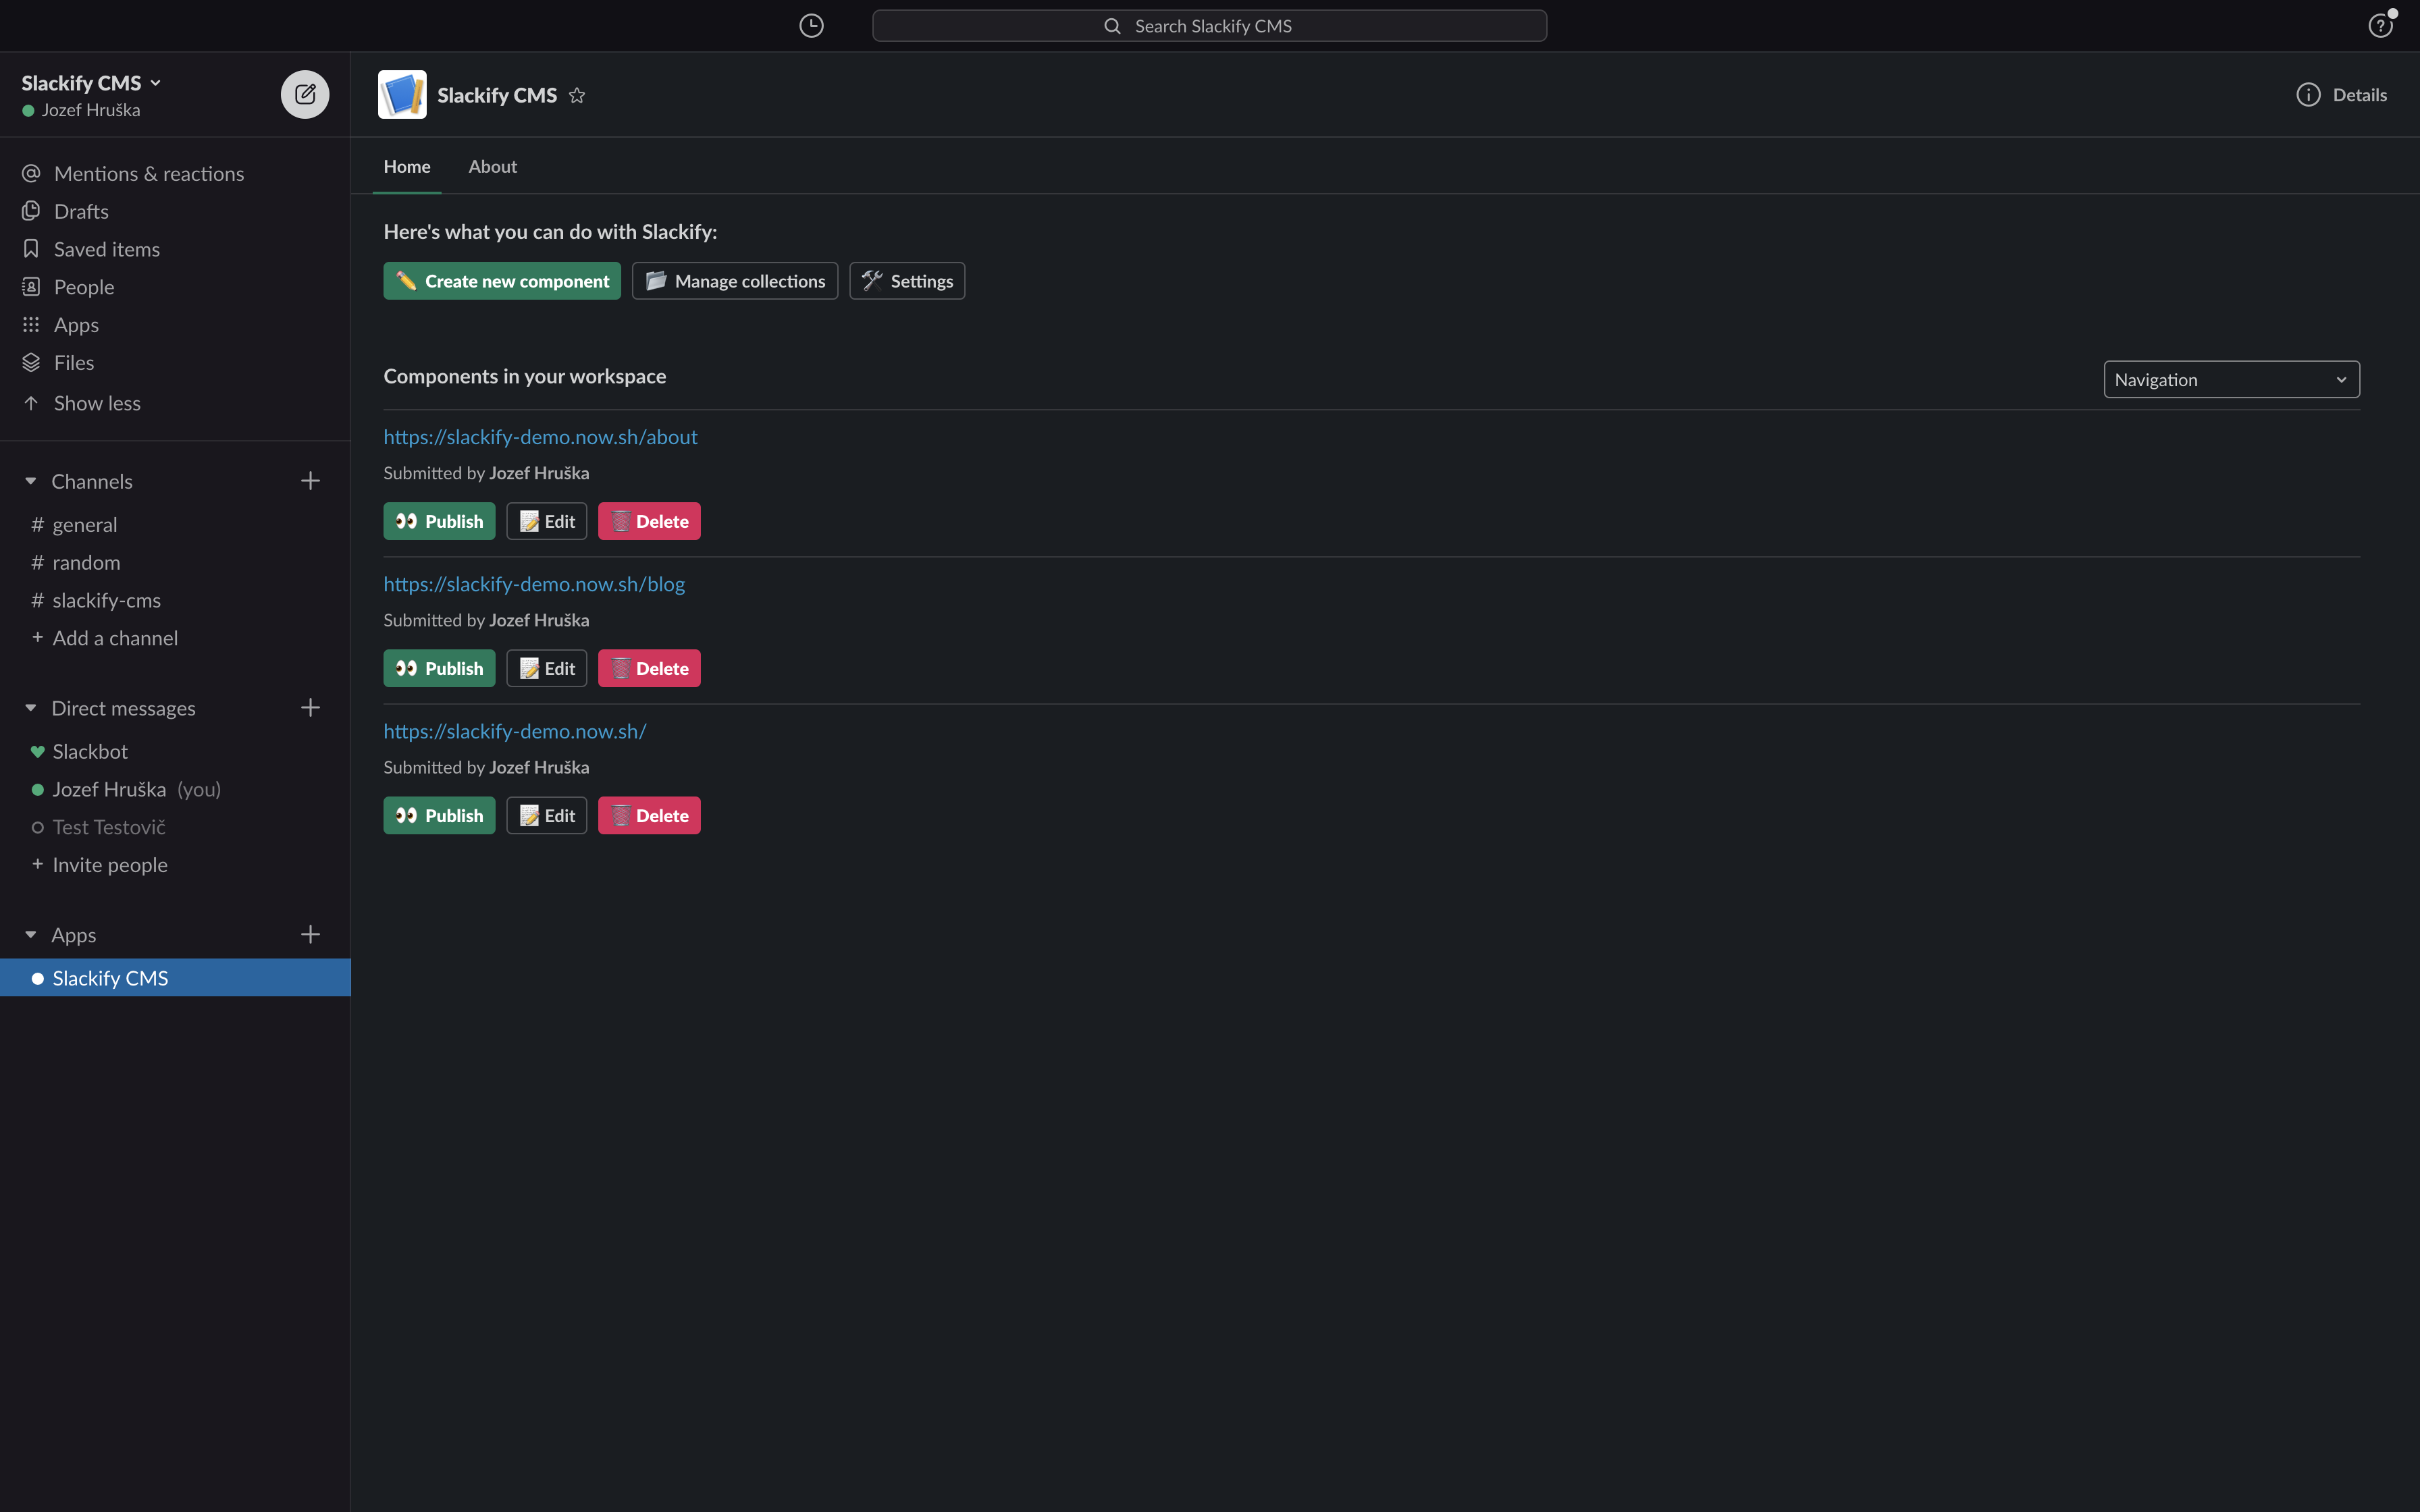
\includegraphics[scale=0.085]{obrazky-figures/screenshot_slack-home}
	\caption{Domovská stránka v~Slack aplikácii.}
\end{figure}

\noindent Na domovskej stránke sa nachádza hlavička so všetkými akciami, ktoré môže užívateľ v~redakčnom systéme vykonávať (ak užívateľ nemá dostatočné práva, akcie sú skryté). Pod touto hlavičkou sa nachádza zoznam komponentov. Zoznam zobrazuje komponenty priradené k~zvolenej kolekcií pomocou elementu \texttt{Select} v~záhlaví zoznamu. Ak nie je zvolená žiadna kolekcia, zobrazuje komponenty priradené k~prvej dostupnej kolekcii. \\

\begin{lstlisting}[caption={Funkcia zodpovedná za generovanie rozhrania domovskej stránky.}]
	async function compose_app_home_view(
		teamId: string,
		userId: string,
		initialCollectionId?: string
	): Promise<View | undefined>
\end{lstlisting}

\medskip

\noindent Domovská stránka je aktualizovaná po rôznych akciách vykonaných užívateľom. Ak užívateľ vytvorí, odstráni alebo upraví kolekciu alebo komponent, rozhranie domovskej stránky musí byť aktualizované s~novými zmenami.

\subsection{Správa kolekcií a komponentov}
Užívateľské rozhranie správy kolekcií a komponentov kopíruje webovú konzolu. Užívateľ má možnosť zobraziť, publikovať, skryť, upraviť a zmazať kolekcie alebo komponenty.

\begin{figure}[h]
	\centering
	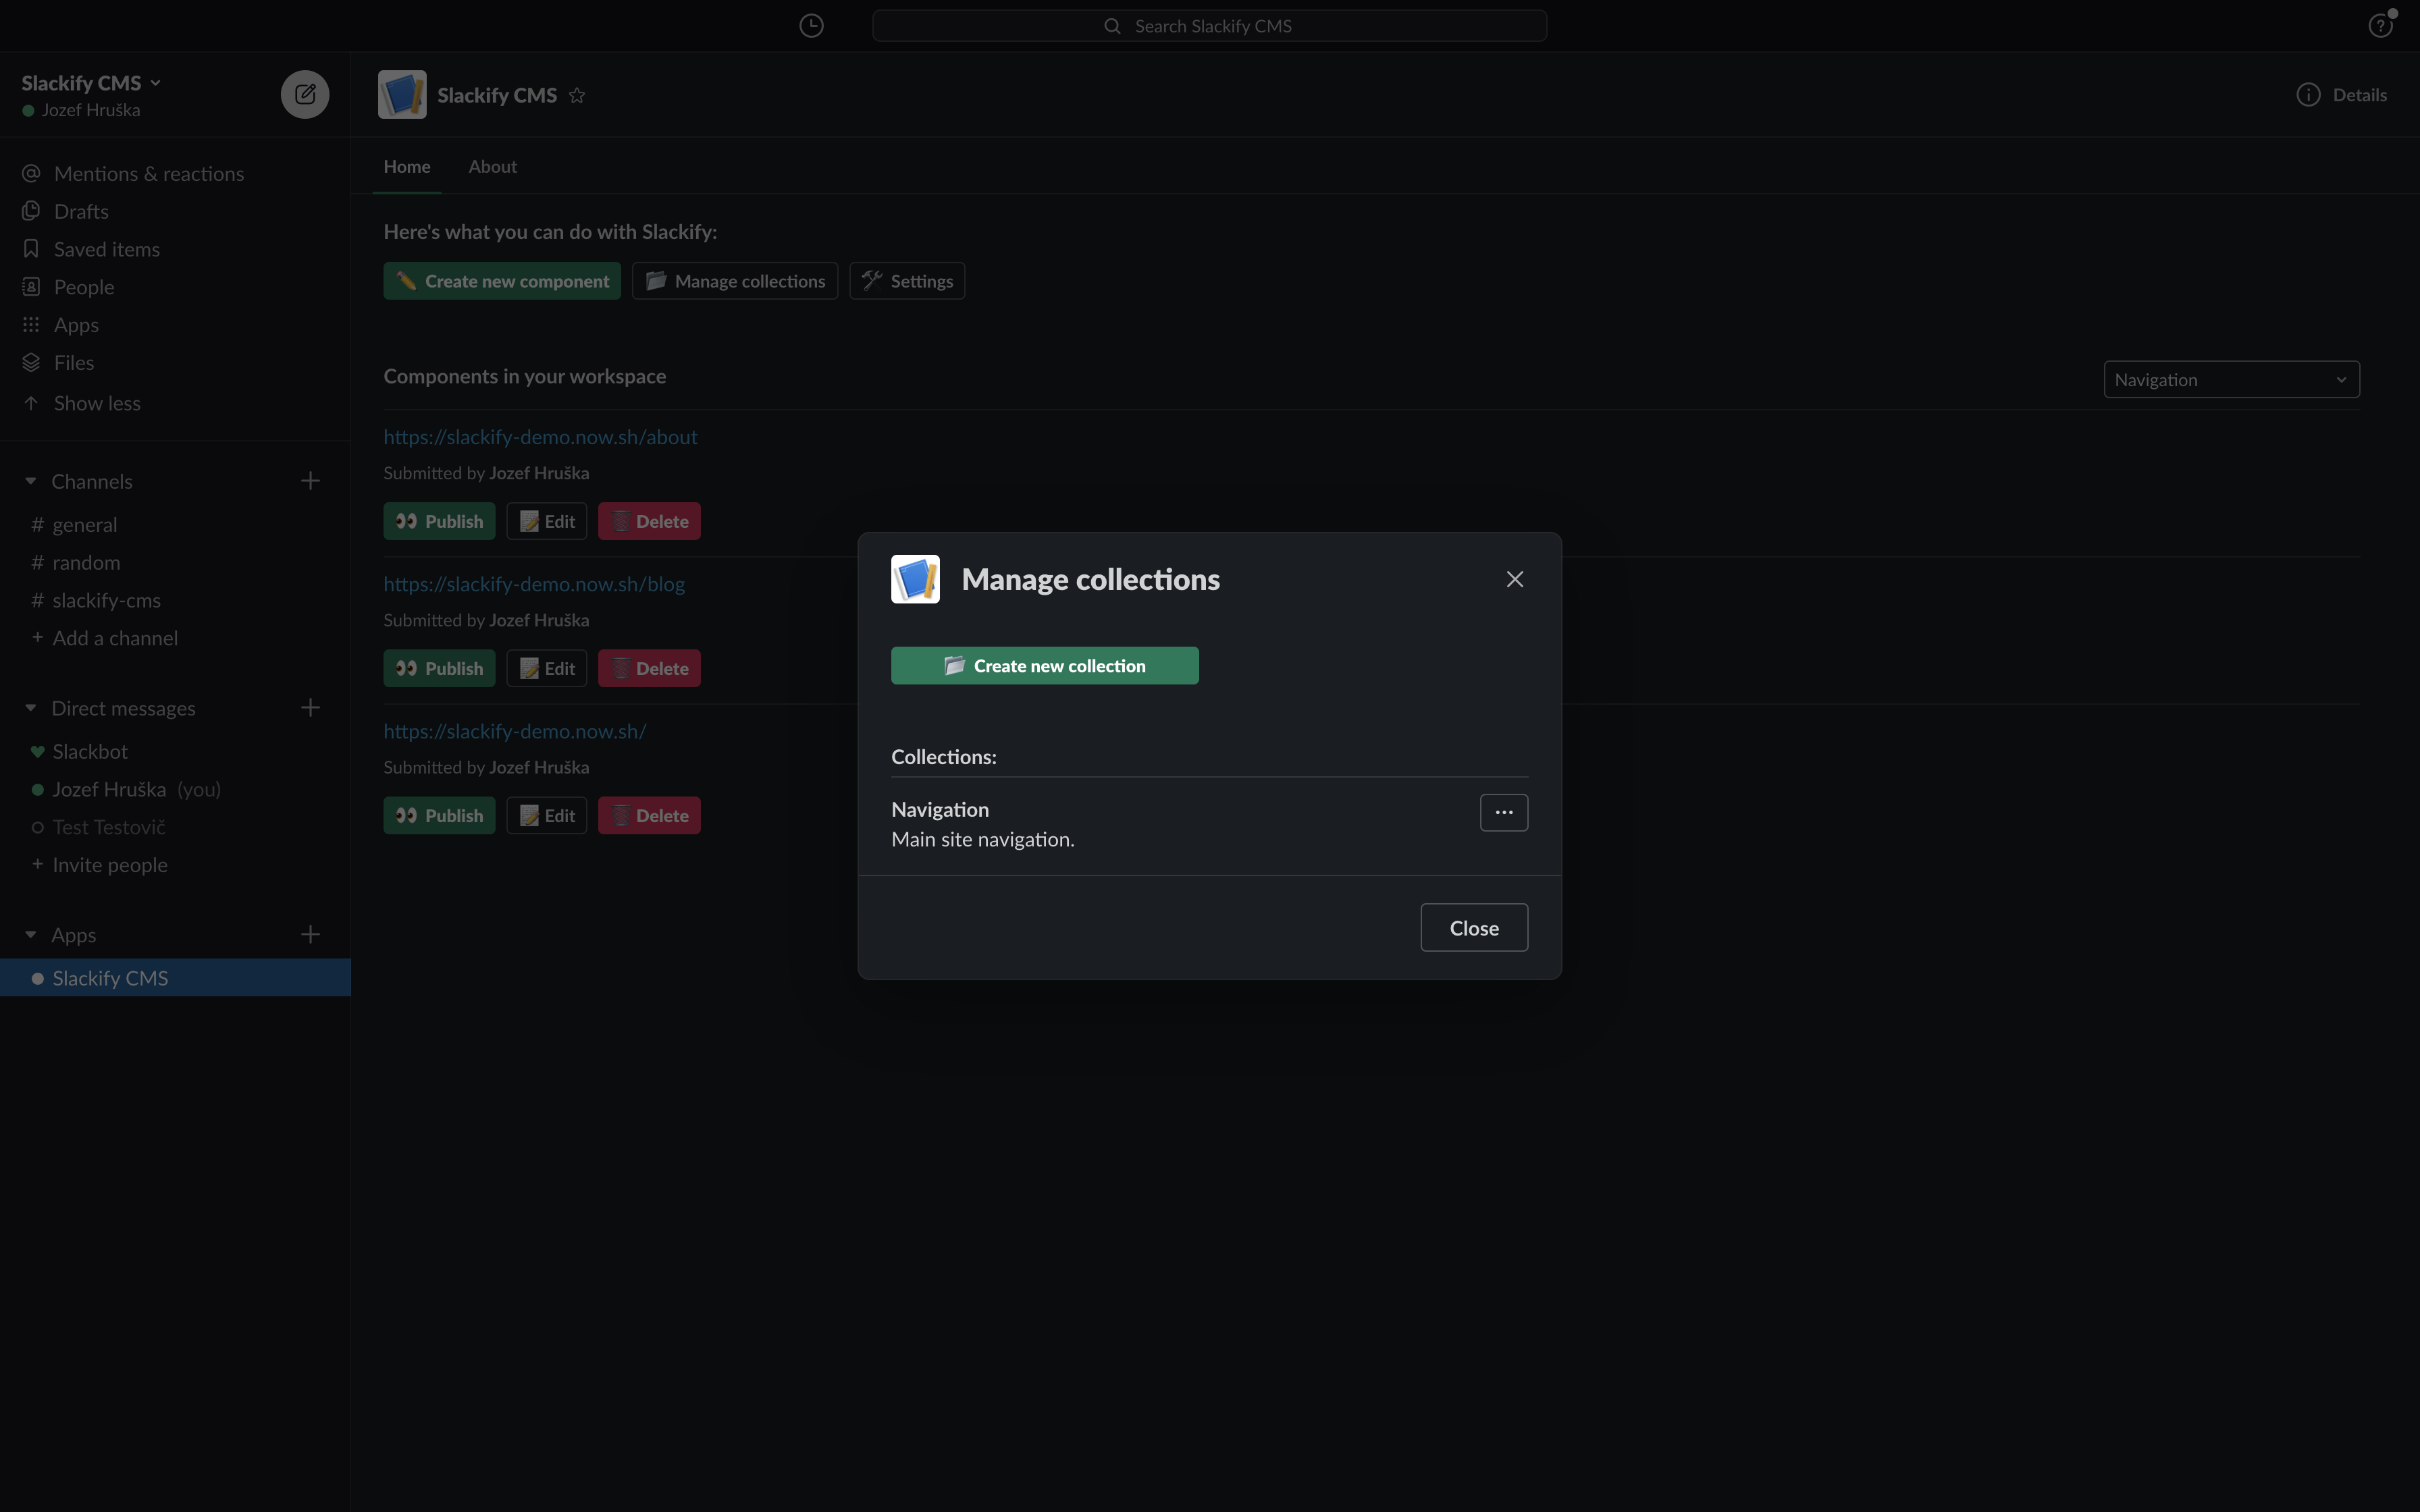
\includegraphics[scale=0.085]{obrazky-figures/screenshot_slack_collections}
	\caption{Dialógové okno so zoznamom kolekcií v~Slack aplikácii.}
\end{figure}

\noindent Zoznam kolekcií sa nachádza v~dialógovom okne prístupnom z~domovskej stránky. Dialógové okná v~Slack aplikácii slúžia pre zobrazovanie informácií, ktoré sa nenachádzajú na domovskej stránke alebo pre získanie dát od užívateľa pomocou formulárov (napríklad vytvorenie novej kolekcie).

% Testovanie
%---------------------------------------------------------------------------
\chapter{Testovanie}
\label{test}
Podstatnou časťou tejto práce bolo testovanie systému. Tak ako end to end a jednotkové testy zabezpečujú správnu funkcionalitu implementácie, tak užívateľské testy pomáhajú odhaľovať nedostatky v~samotnom používaní systému.

Táto kapitola je venovaná užívateľskému testovaniu headless redakčného systému Slackify. Prvá sekcia \ref{test:dev} popisuje princíp a závery z~testovania počas implementovania samotným vývojárom a druhá sekcia \ref{test:user} sa venuje užívateľskému testovaniu osobami, ktoré sa na vývoji nepodieľali.

\section{Testovanie počas vývoja}
\label{test:dev}
Testovanie počas vývoja je prirodzeným procesom pri navrhovaní a implementovaní softvéru. Pri každom zásahu do návrhu alebo implementácie bola každá zmena užívateľsky testovaná vývojárom. Ak neboli splnené požiadavky na funkčnosť, postupnými iteráciami nad návrhom alebo implementáciou boli problémy identifikované a odstránené.

\section{Užívateľské testovanie}
\label{test:user}
Headless redakčné systémy vyžadujú pre ich používanie pokročilejšie technické znalosti. Z~tohto dôvodu bola pre testovanie zvolená osoba pôsobiaca v~oblasti IT a vývoja.

\subsection{Testovacie scenáre}
Testovacie scenáre boli zostavené z~najbežnejších úkonov, ktoré by typický užívateľ v~systéme vykonával. Testovanie prebiehalo za minimálneho zásahu osôb, ktoré neboli jeho súčasťou. Z~dôvodu minimálnej užívateľskej dokumentácie však malé zásahy boli potrebné. \\

\noindent Úspech každého testovacieho scenáru bol vyhodnotený jednou z~troch možností:

\begin{itemize}
	\item \texttt{ÁNO} -- Úspech
	\item \texttt{NIE} -- Neúspech
	\item \texttt{$\varnothing$} -- Čiastočný úspech / Čiastočný neúspech
\end{itemize}

\begin{center}
	{\renewcommand{\arraystretch}{1.4}%
	\begin{tabularx}{\textwidth}{ | c | X | c | }
		\hline
		\rowcolor{lightgray} \multicolumn{3}{| c |}{Webová konzola} \\
		\hline
		& Názov & Úspech \\
		\hline
		\hline
		1. & \textbf{Pridanie Slackify do pracovného prostredia v~Slacku} \newline Poznámka: Chýbajúce zdôvodnenie požadovaných oprávnení. & ÁNO \\
		\hline
		2. & \textbf{Prihlásenie sa do užívateľského účtu} & ÁNO \\
		\hline
		3. & \textbf{Vytvorenie kolekcie} \newline Poznámka: Chýbajúce označenie voliteľných polí. & ÁNO \\
		\hline
		4. & \textbf{Vytvorenie komponentu} \newline Poznámka: Chýbajúca možnosť vytvoriť komponent priamo v~detaile kolekcie & ÁNO \\
		\hline
		5. & \textbf{Odstránenie komponentu} & ÁNO \\
		\hline
		5. & \textbf{Odstránenie kolekcie} & ÁNO \\
		\hline
	\end{tabularx}}
\end{center}

\begin{center}
	{\renewcommand{\arraystretch}{1.4}%
	\begin{tabularx}{\textwidth}{ | c | X | c | }
		\hline
		\rowcolor{lightgray} \multicolumn{3}{| c |}{Slack aplikácia} \\
		\hline
		& Názov & Úspech \\
		\hline
		\hline
		1. & \textbf{Vytvorenie kolekcie} \newline Poznámka: Odhalená chyba v~zobrazení zoznamu komponentov typu \texttt{Article} s~nevyplneným poľom \uv{lead}. Chýbajúce upozornenie pri duplicite názvov kolekcií. & ÁNO \\
		\hline
		2. & \textbf{Vytvorenie komponentu} & ÁNO \\
		\hline
		3. & \textbf{Odstránenie komponentu} \newline Poznámka: Chýbajúce potvrdenie pri zmazaní komponentu. & ÁNO \\
		\hline
		4. & \textbf{Odstránenie kolekcie} \newline Poznámka: Chýbajúce potvrdenie pri zmazaní kolekcie. & ÁNO \\
		\hline
	\end{tabularx}}
\end{center}

\begin{center}
	{\renewcommand{\arraystretch}{1.4}%
	\begin{tabularx}{\textwidth}{ | c | X | c | }
		\hline
		\rowcolor{lightgray} \multicolumn{3}{| c |}{Verejné GraphQL rozhranie} \\
		\hline
		& Názov & Úspech \\
		\hline
		\hline
		1. & \textbf{Získanie všetkých kolekcií} & ÁNO \\
		\hline
		2. & \textbf{Získanie jednej kolekcie} & ÁNO \\
		\hline
		3. & \textbf{Získanie všetkých komponentov v~kolekcii} & ÁNO \\
		\hline
		4. & \textbf{Získanie jedného komponentu} & ÁNO \\
		\hline
	\end{tabularx}}
\end{center}

\subsection{Záver užívateľského testovania}
Všetky scenáre užívateľského testovania boli \emph{úspešné} aj vďaka silnému dôrazu na prívetivosť užívateľského rozhrania pri vývoji. Pri testovaní boli odhalené malé nedostatký návrhu alebo implementácie systému uvedené v~poznámke pri danom testovacom scenári.

% Záver
%---------------------------------------------------------------------------
\chapter{Záver}
\label{conc}
Cieľom práce bolo vytvoriť headless redakčný systém s~možnosťou správy obsahu v~službe Slack. Výsledné riešenie, redakčný systém Slackify, splňuje všetky body formálneho zadania s~výnimkou využitia aplikácie Slack pre ukladanie dát. Už pri návrhu riešenia som odhalil niekoľko prekážok, pre ktoré som sa rozhodol, že obsah redakčného systému bude ukladaný v~konvenčnej databáze.

Na začiatku práce som analyzoval existujúce headless redakčné systémy a nedostatky v~ich nasadení, používaní alebo architektúre. Slackify adresuje a rieši tieto nedostatky. Umožňuje užívateľom spravovať a distribuovať obsah bez zbytočnej komplexity súčasných riešení, čo považujem za hlavný úspech tejto práce.

Vďaka tejto práci som sa naučil budovať robustné systémy a serverové aplikácie. Oblasť, v~ktorej som nemal pred touto prácou žiadne skúsenosti a minimálne znalosti. Toto rozhodnutie spravilo prácu náročnejšou, ale o~to viac odmeňujúcou.

Jedným z~možných rozšírení, ktorého implementáciu som sám zvažoval je možnosť definovať vlastné typy komponentov. Toto rozšírenie by značne zvýšilo flexibilitu systému, no zároveň by si rozporovalo s~hlavným cieľom tejto práce -- jednoduchosťou použitia.
 
  % Pouzita literatura / Bibliography
  % ----------------------------------------------
\ifslovak
  \makeatletter
  \def\@openbib@code{\addcontentsline{toc}{chapter}{Literatúra}}
  \makeatother
  \bibliographystyle{bib-styles/Pysny/skplain}
\else
  \ifczech
    \makeatletter
    \def\@openbib@code{\addcontentsline{toc}{chapter}{Literatura}}
    \makeatother
    \bibliographystyle{bib-styles/Pysny/czplain}
  \else 
    \makeatletter
    \def\@openbib@code{\addcontentsline{toc}{chapter}{Bibliography}}
    \makeatother
    \bibliographystyle{bib-styles/Pysny/enplain}
  %  \bibliographystyle{alpha}
  \fi
\fi
  \begin{flushleft}
  \bibliography{xhrusk25-slack-api-headless-cms-20-literatura-bibliography}
  \end{flushleft}

  % vynechani stranky v oboustrannem rezimu
  % Skip the page in the two-sided mode
  \iftwoside
    \cleardoublepage
  \fi

  % Prilohy / Appendices
  % ---------------------------------------------
  \appendix
\ifczech
  \renewcommand{\appendixpagename}{Přílohy}
  \renewcommand{\appendixtocname}{Přílohy}
  \renewcommand{\appendixname}{Příloha}
\fi
\ifslovak
  \renewcommand{\appendixpagename}{Prílohy}
  \renewcommand{\appendixtocname}{Prílohy}
  \renewcommand{\appendixname}{Príloha}
\fi
%  \appendixpage

% vynechani stranky v oboustrannem rezimu
% Skip the page in the two-sided mode
%\iftwoside
%  \cleardoublepage
%\fi
  
\ifslovak
%  \section*{Zoznam príloh}
%  \addcontentsline{toc}{section}{Zoznam príloh}
\else
  \ifczech
%    \section*{Seznam příloh}
%    \addcontentsline{toc}{section}{Seznam příloh}
  \else
%    \section*{List of Appendices}
%    \addcontentsline{toc}{section}{List of Appendices}
  \fi
\fi
  \startcontents[chapters]
  \setlength{\parskip}{0pt} 
  % seznam příloh / list of appendices
  % \printcontents[chapters]{l}{0}{\setcounter{tocdepth}{2}}
  
  \ifODSAZ
    \setlength{\parskip}{0.5\bigskipamount}
  \else
    \setlength{\parskip}{0pt}
  \fi
  
  % vynechani stranky v oboustrannem rezimu
  \iftwoside
    \cleardoublepage
  \fi
  
  % Přílohy / Appendices
  % Tento soubor nahraďte vlastním souborem s přílohami (nadpisy níže jsou pouze pro příklad)

% Umístění obsahu paměťového média do příloh je vhodné konzultovat s vedoucím
%\chapter{Obsah přiloženého paměťového média}

%\chapter{Manuál}

%\chapter{Konfigurační soubor}

%\chapter{RelaxNG Schéma konfiguračního souboru}

%\chapter{Plakát}
  
  % Kompilace po částech (viz výše, nutno odkomentovat)
  % Compilation piecewise (see above, it is necessary to uncomment it)
  %\subfile{xhrusk25-slack-api-headless-cms-30-prilohy-appendices}
  
\end{document}
